\chapter{\label{app:sec:logscale}Simultaneous fit plot with log scale}

\minitoc

\begin{sidewaysfigure}[h]
\centering
\subfloat[$K\pi$, LL]{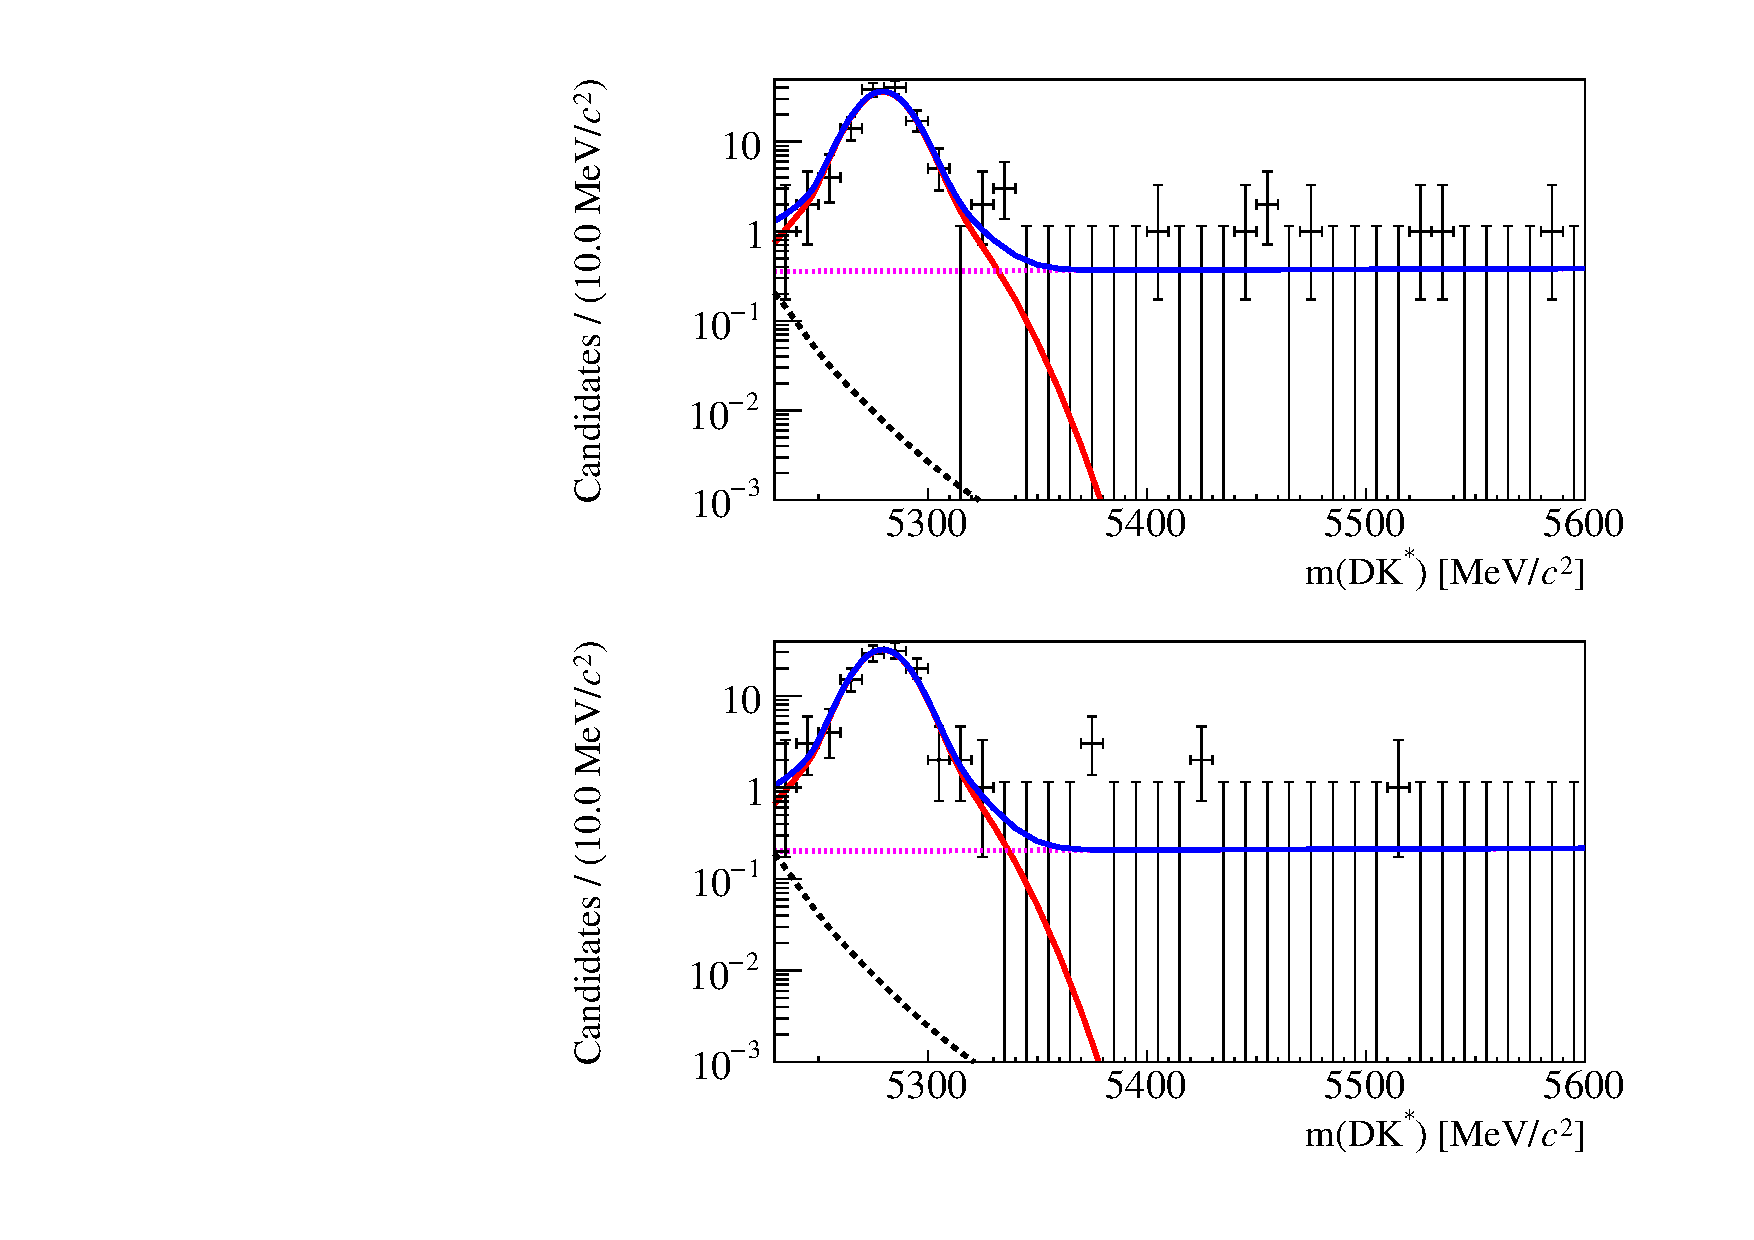
\includegraphics[width=0.25\linewidth]{figures/results/canvaslog_d2kpi_LL_run1_log.pdf}}
\hfill
\subfloat[$KK$, LL]{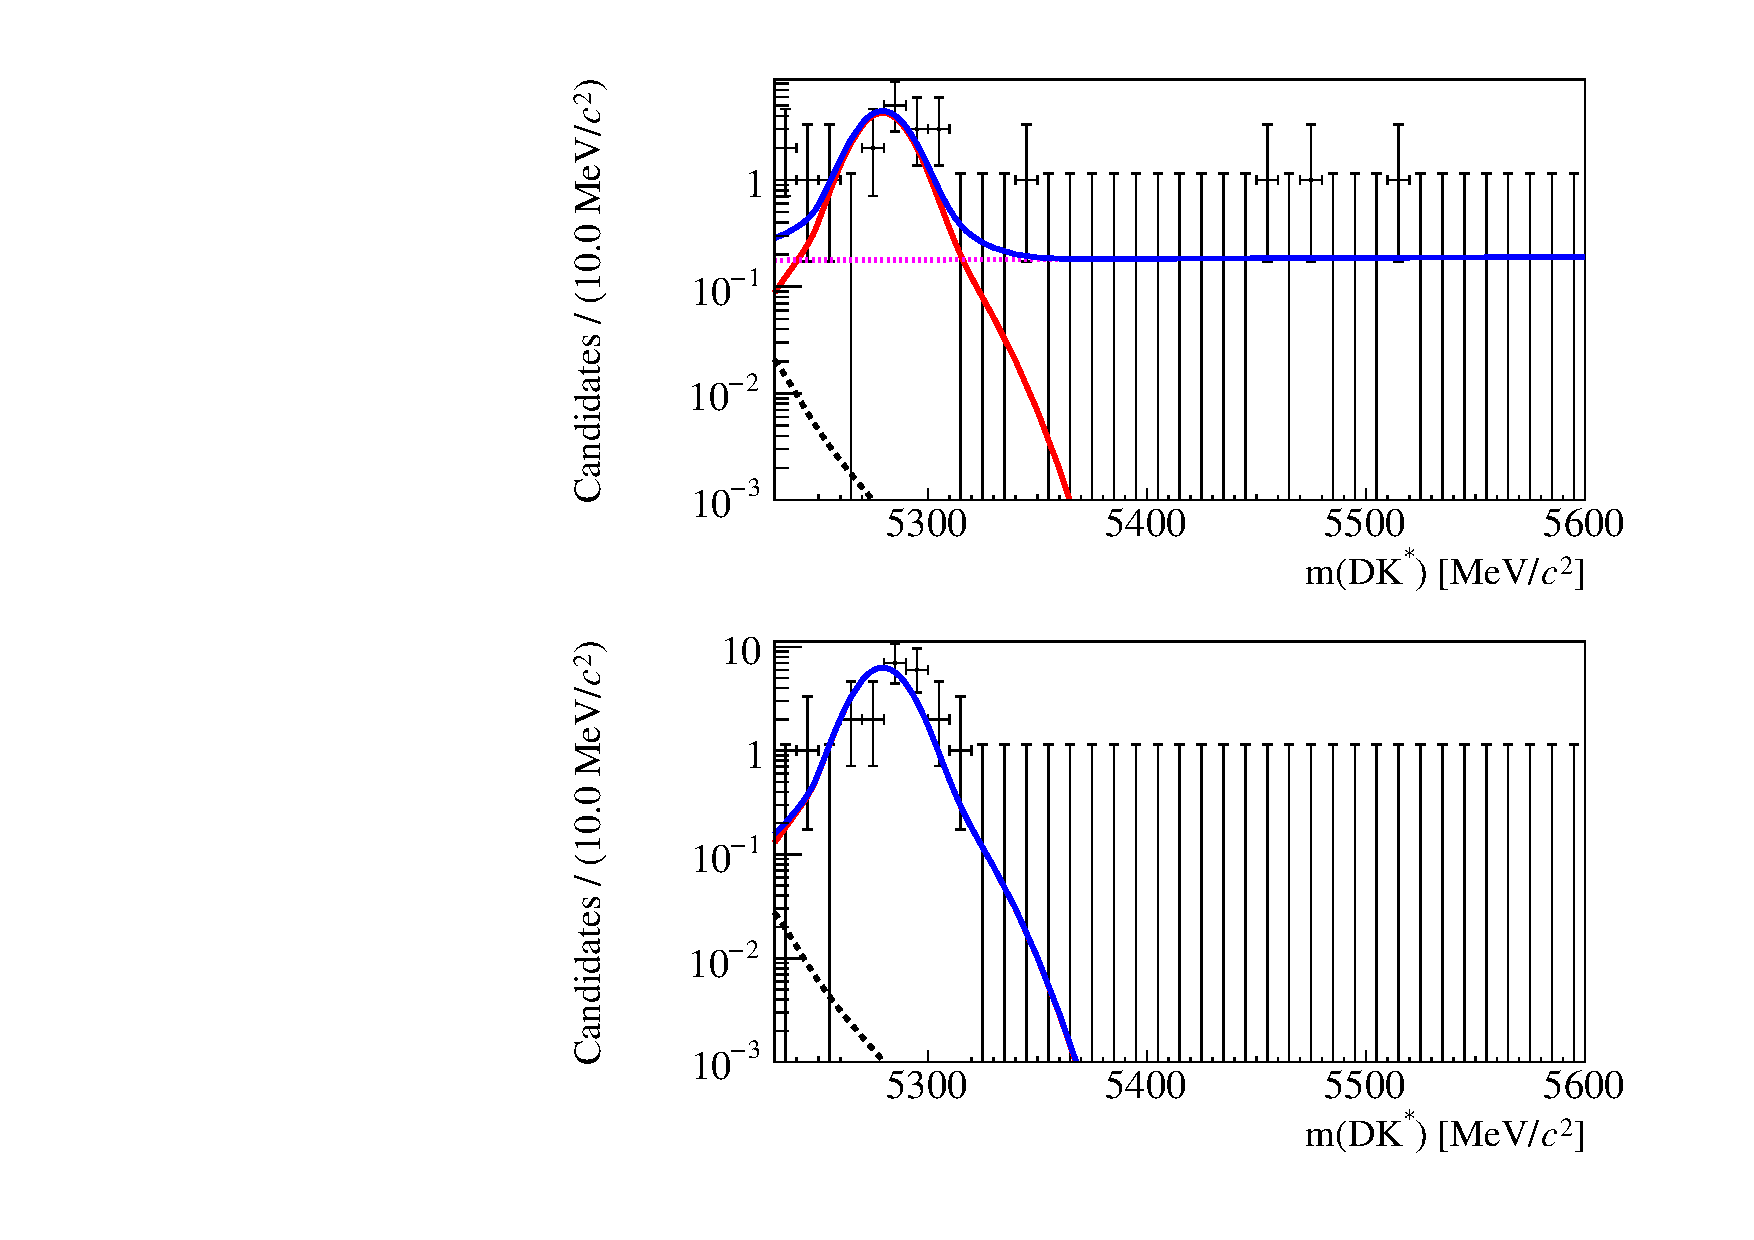
\includegraphics[width=0.25\linewidth]{figures/results/canvaslog_d2kk_LL_run1_log.pdf}}
\hfill
\subfloat[$\pi\pi$, LL]{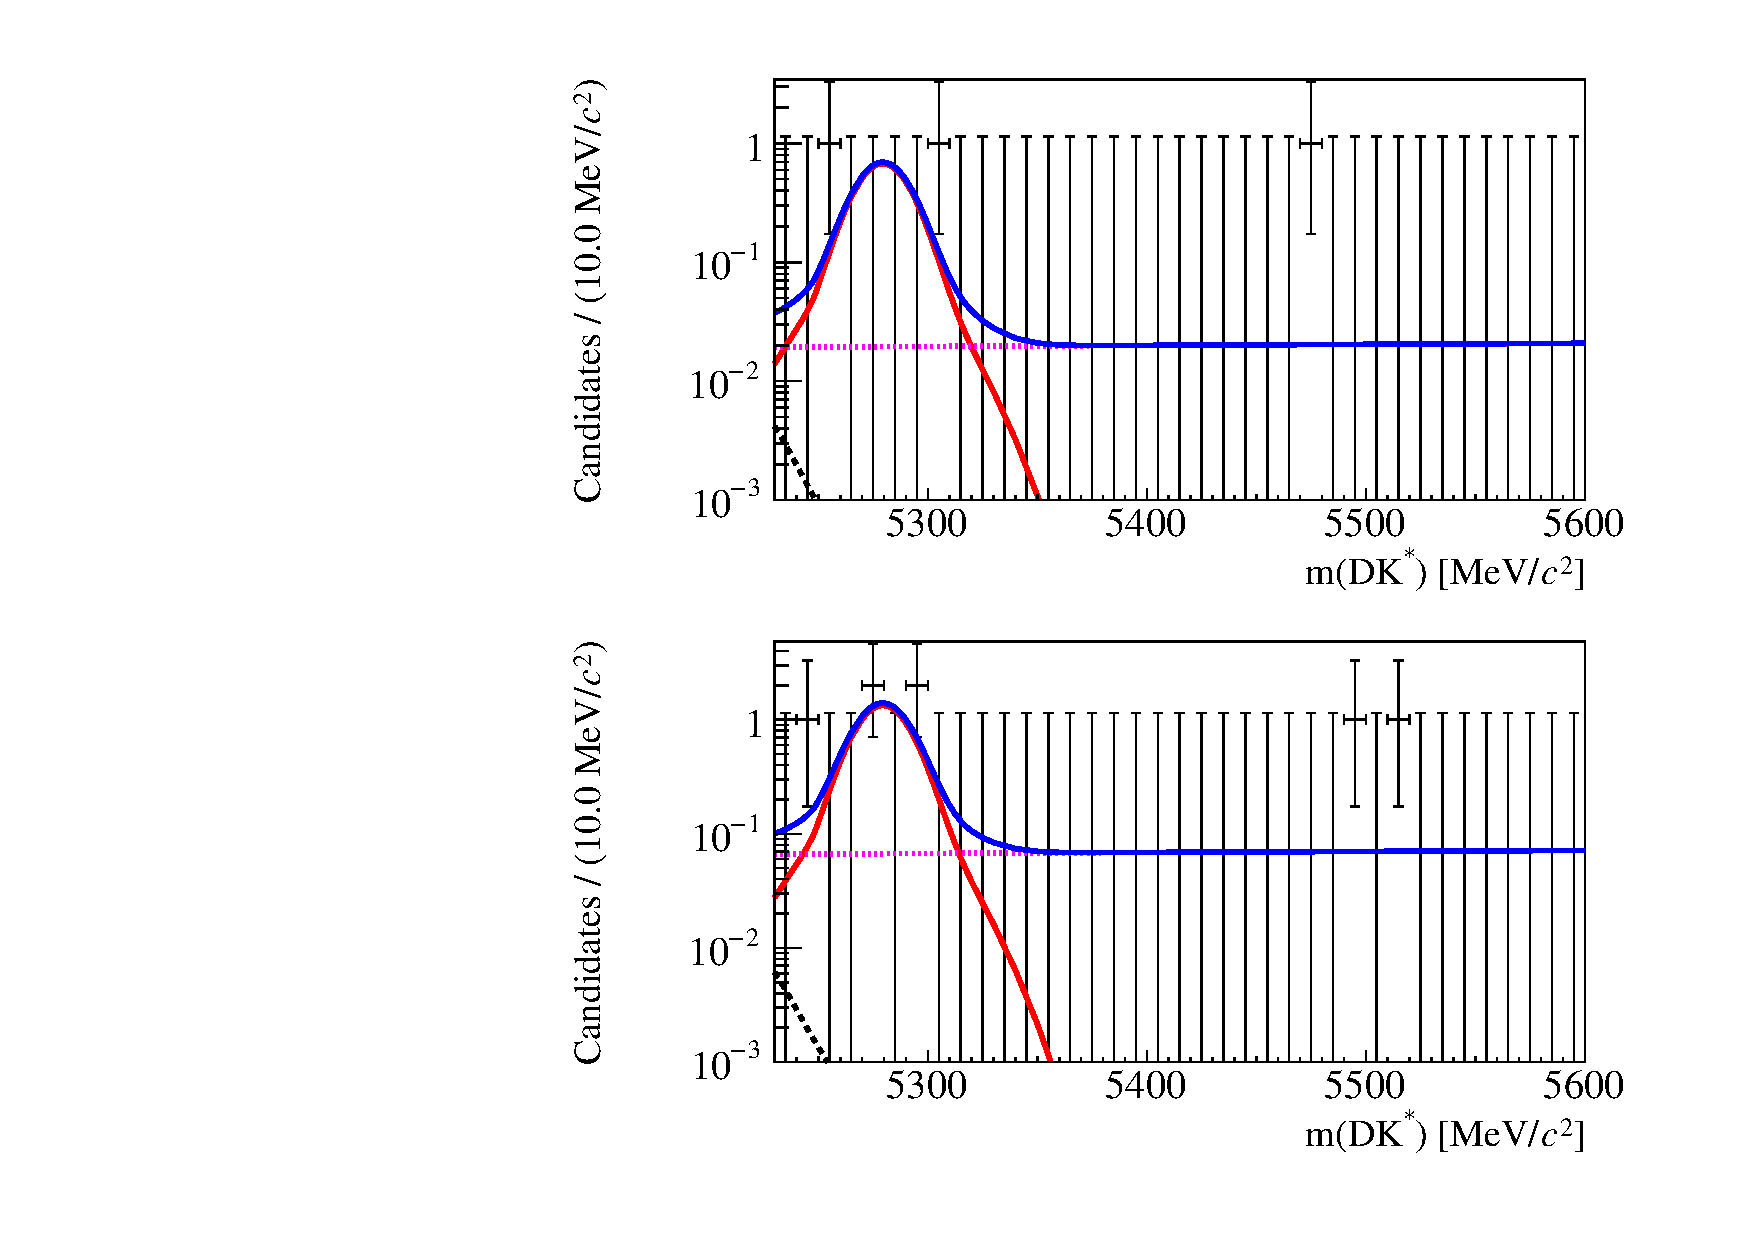
\includegraphics[width=0.25\linewidth]{figures/results/canvaslog_d2pipi_LL_run1_log.pdf}}
\hfill
\subfloat[$\pi K$, LL]{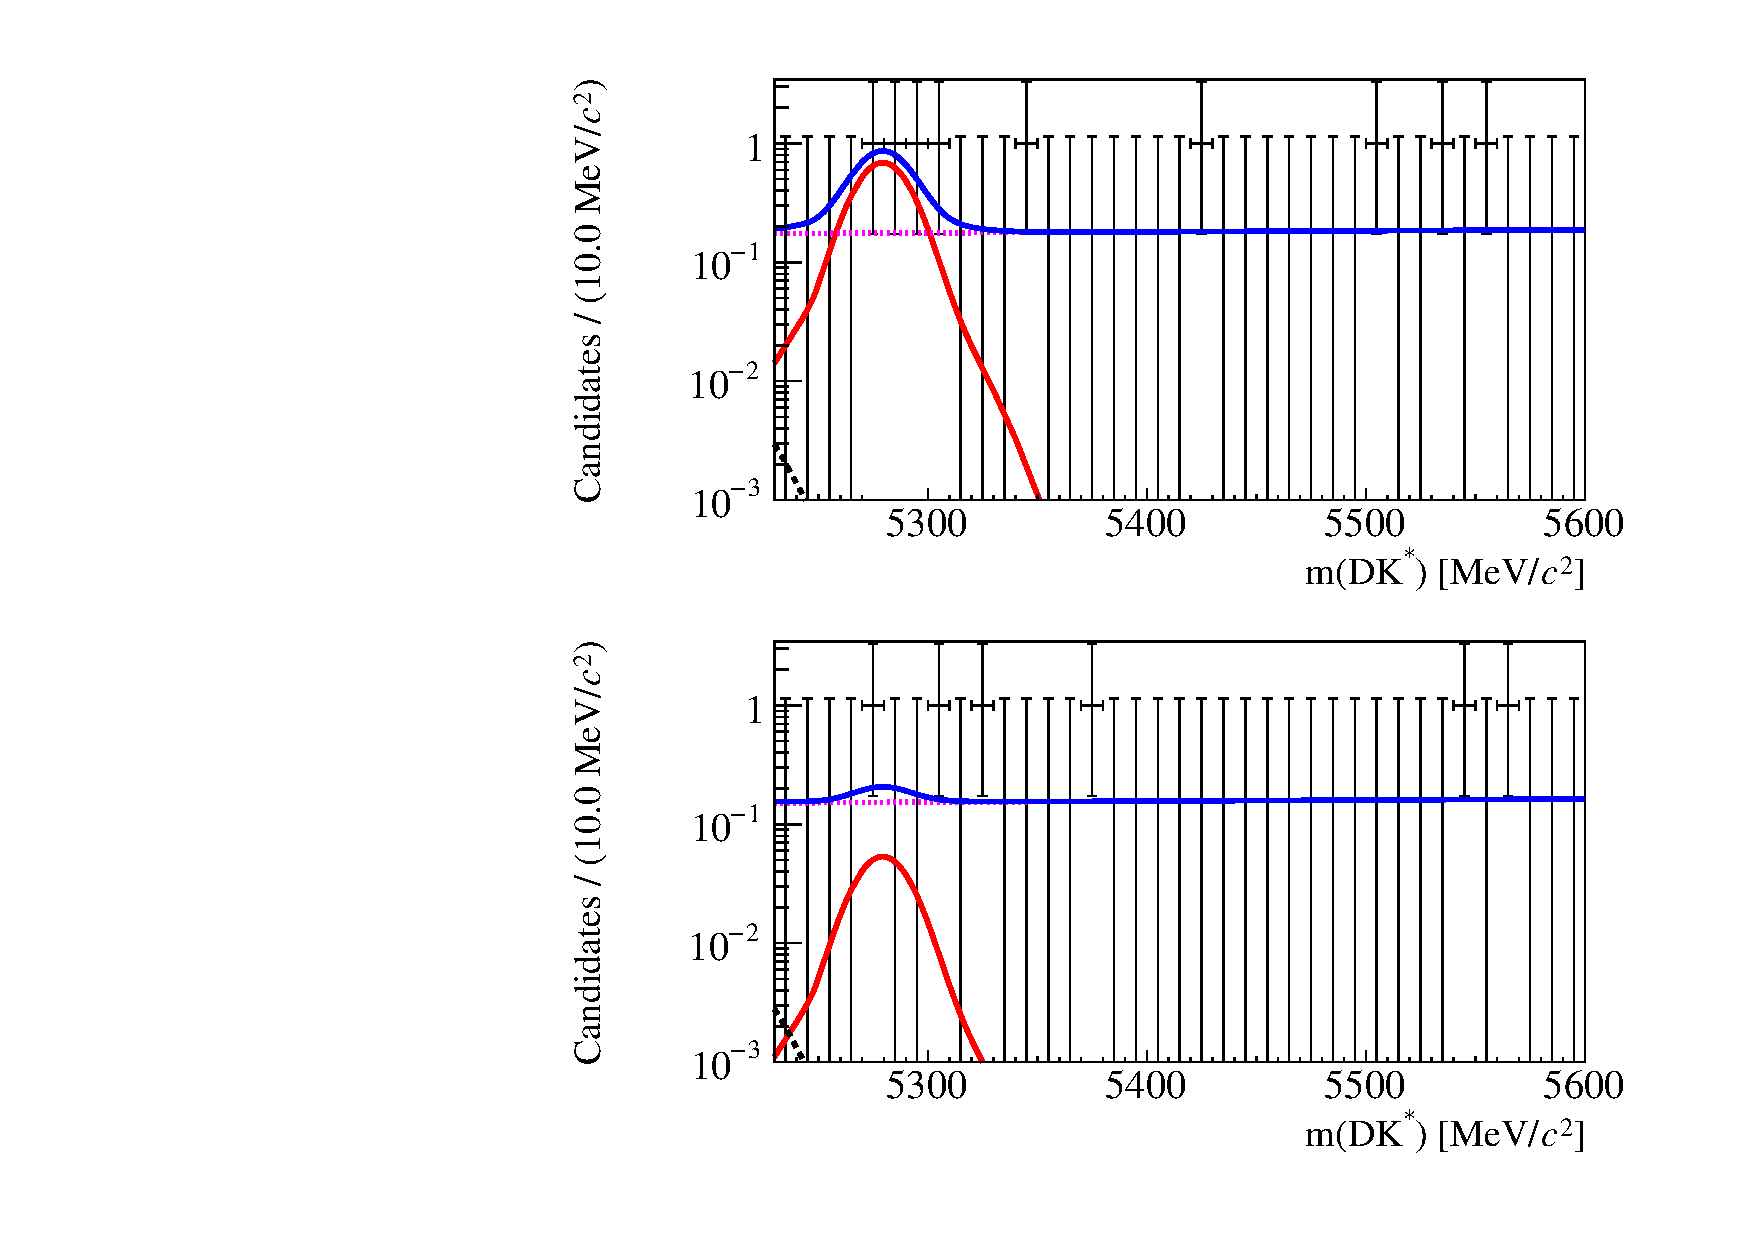
\includegraphics[width=0.25\linewidth]{figures/results/canvaslog_d2pik_LL_run1_log.pdf}}
\hfill
\subfloat[$K\pi$, DD]{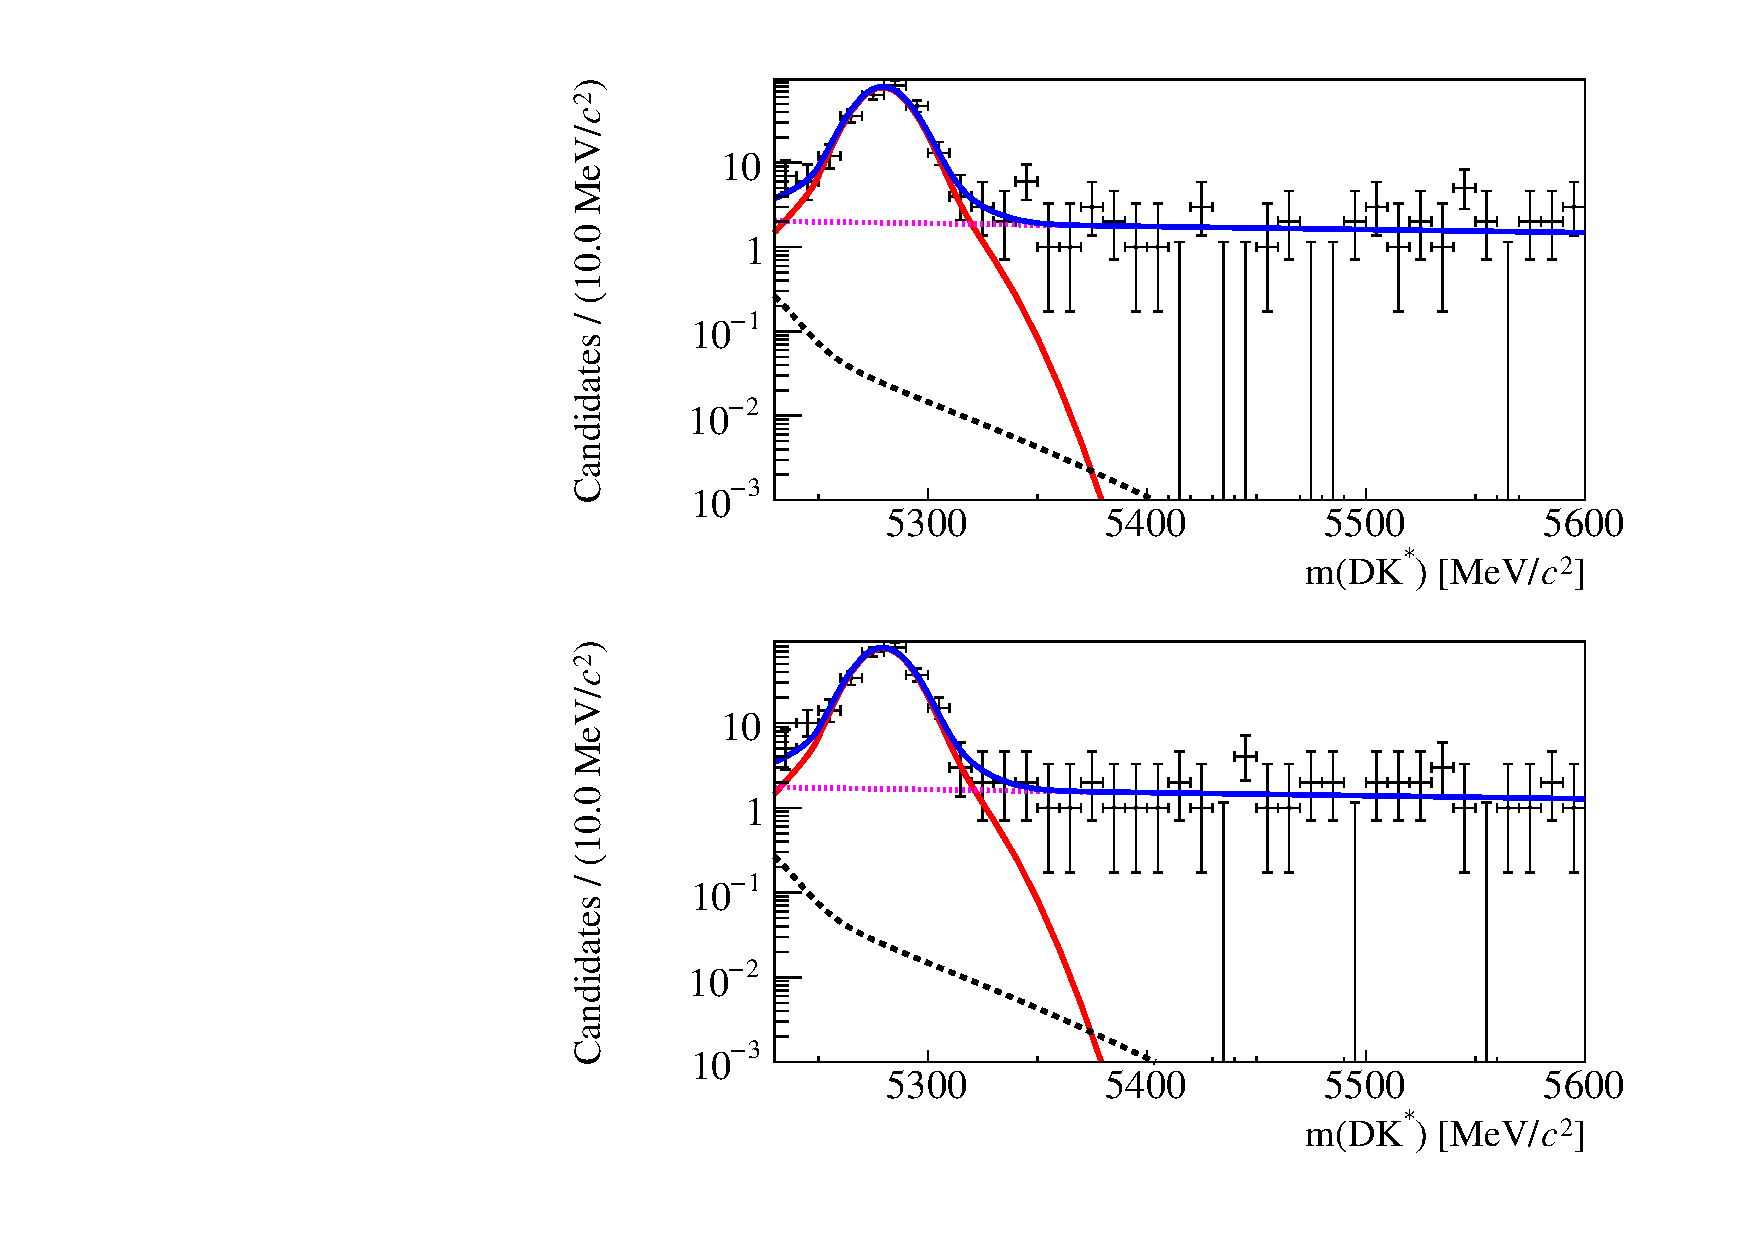
\includegraphics[width=0.25\linewidth]{figures/results/canvaslog_d2kpi_DD_run1_log.pdf}}
\hfill
\subfloat[$KK$, DD]{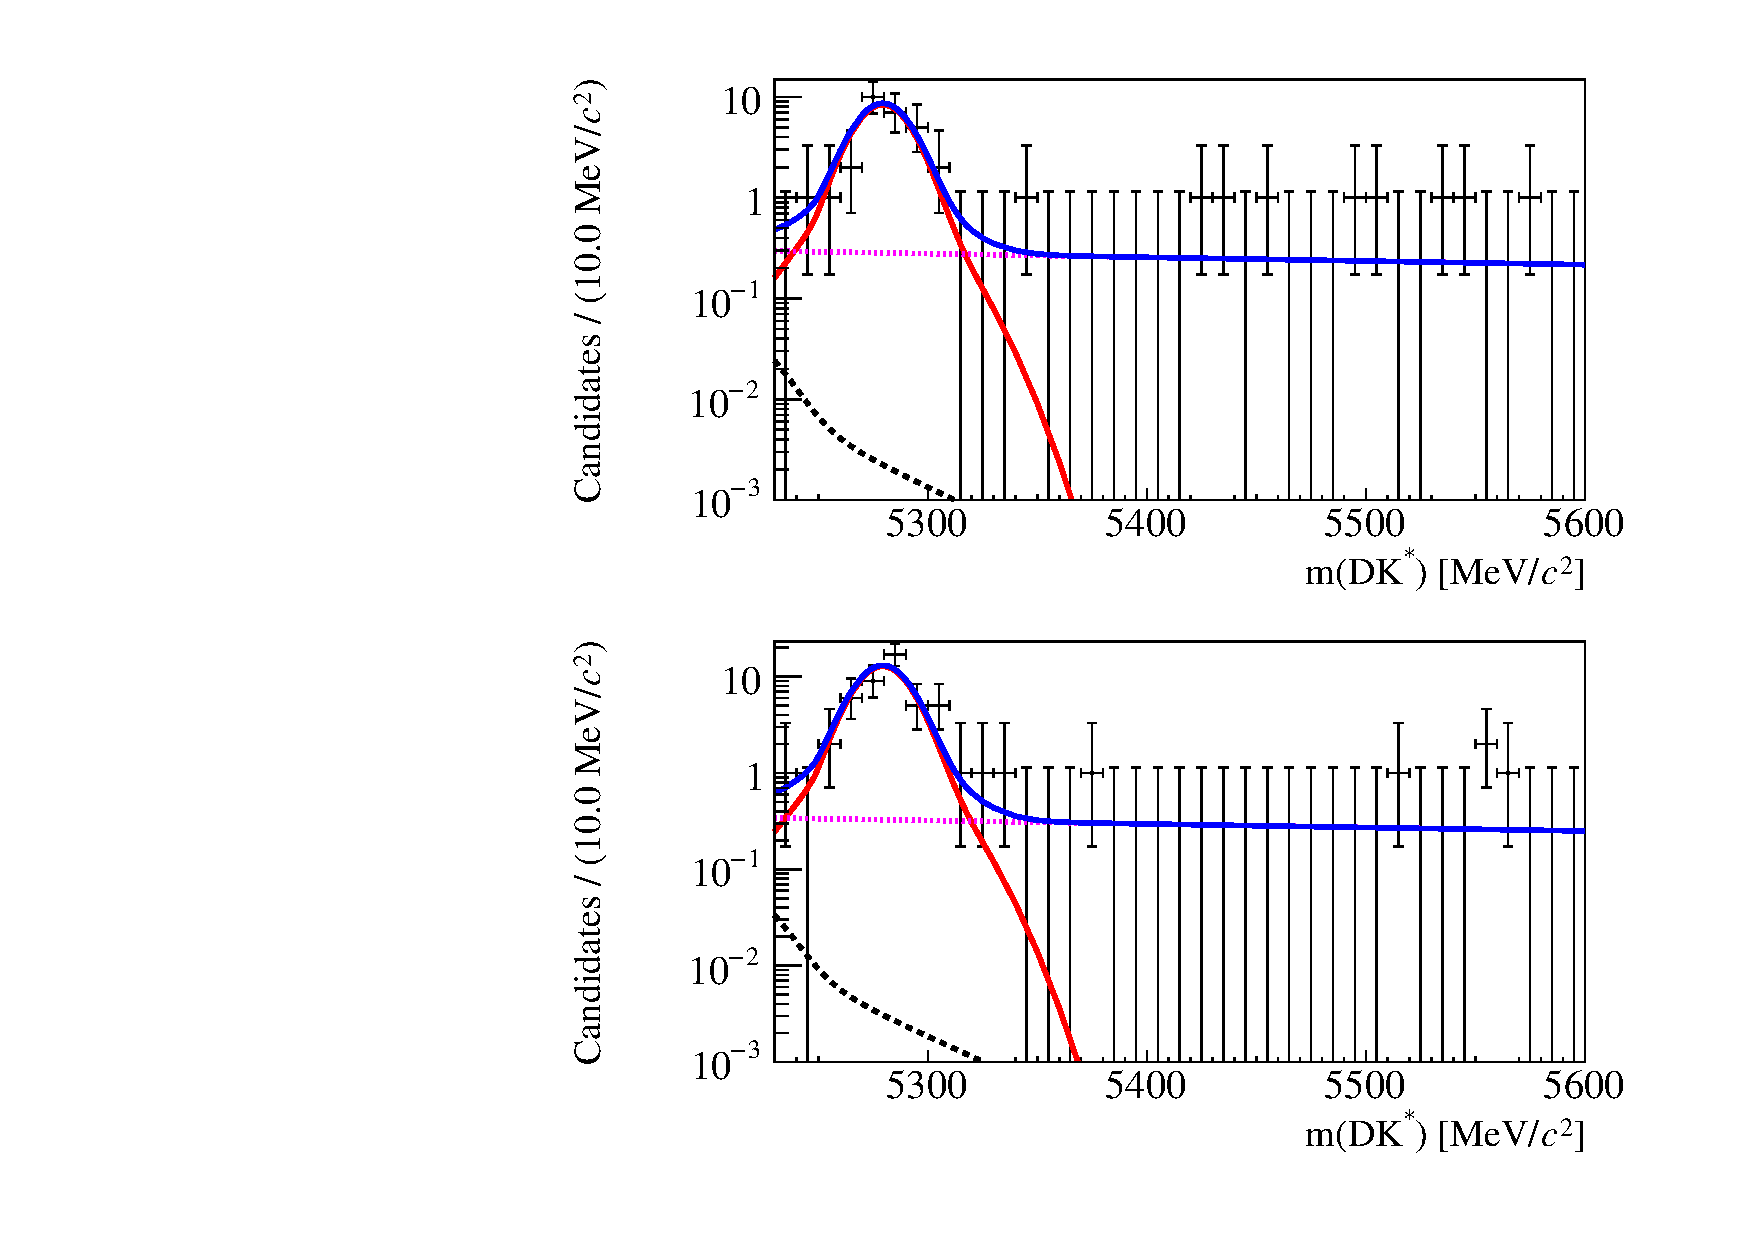
\includegraphics[width=0.25\linewidth]{figures/results/canvaslog_d2kk_DD_run1_log.pdf}}
\hfill
\subfloat[$\pi\pi$, DD]{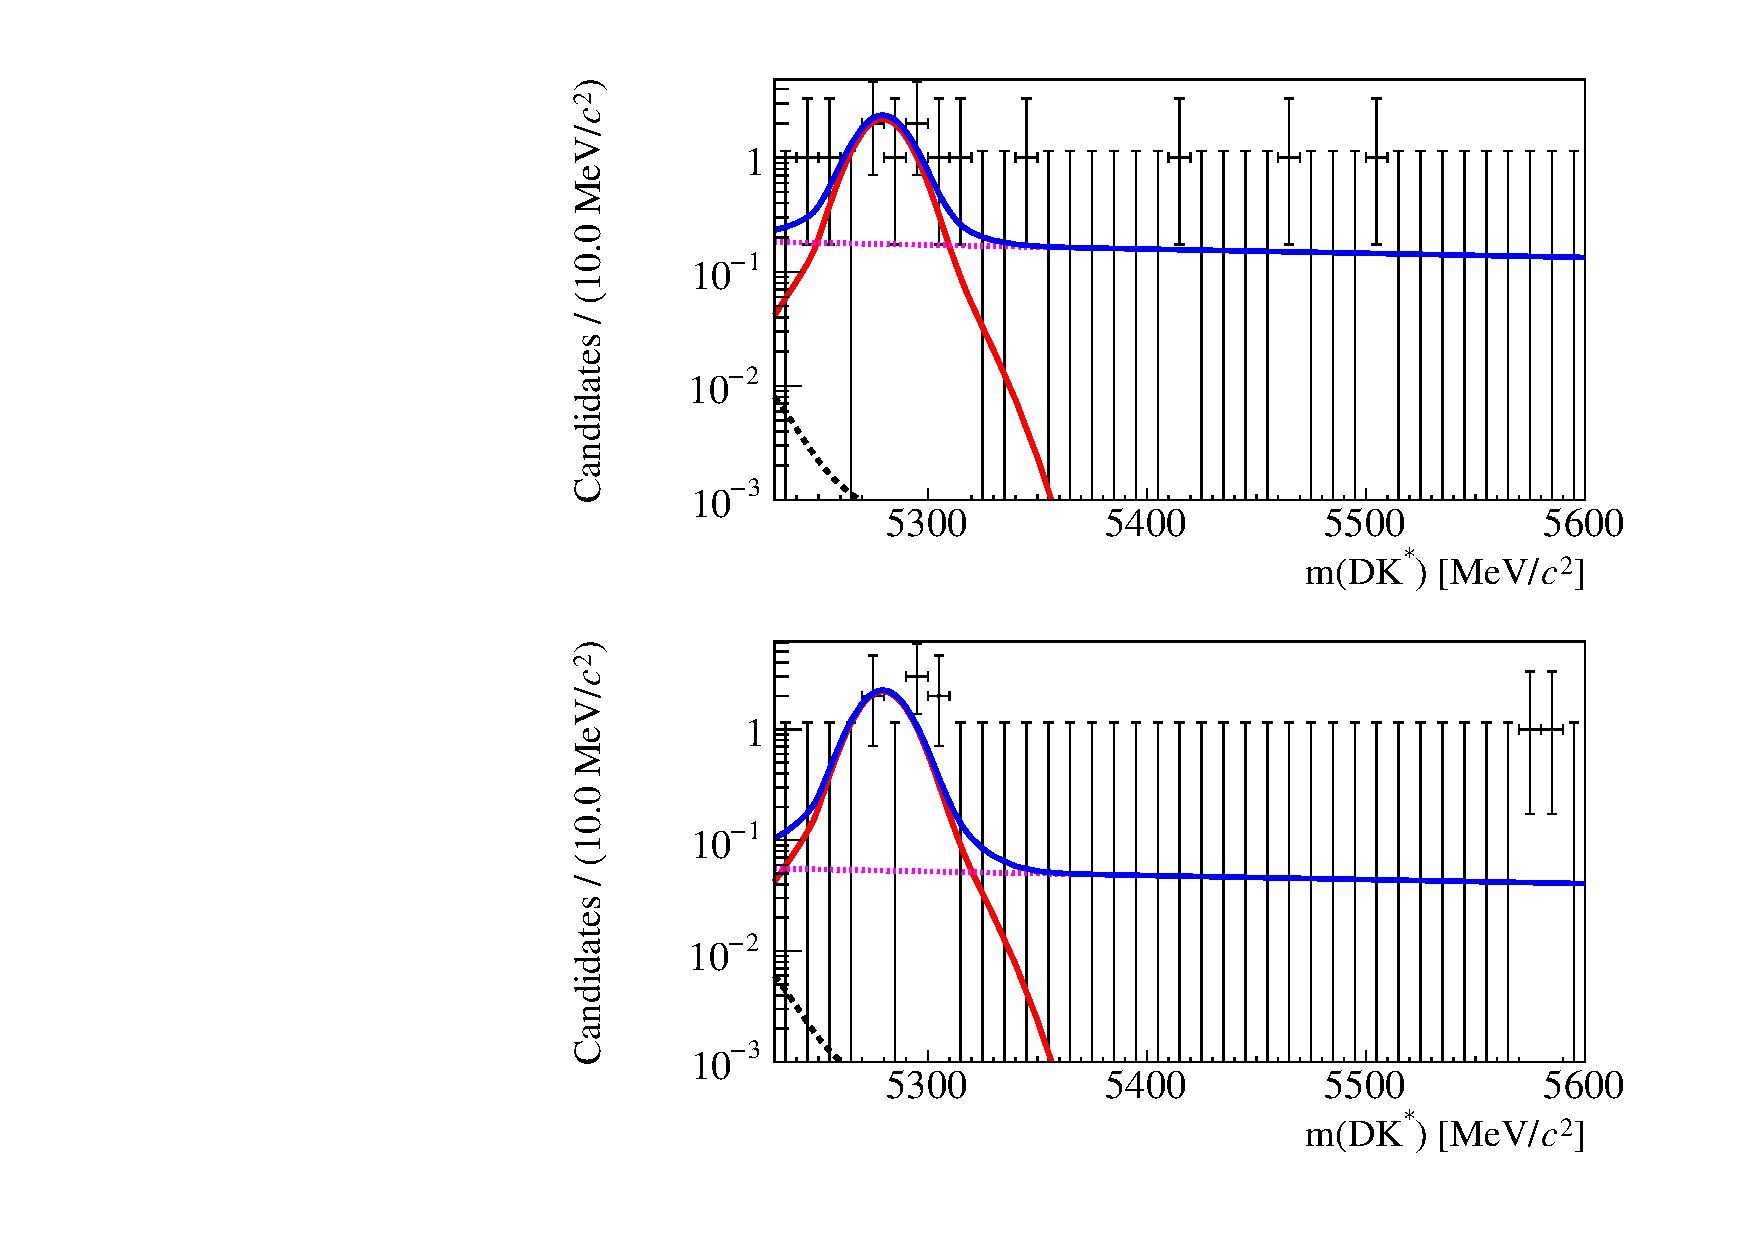
\includegraphics[width=0.25\linewidth]{figures/results/canvaslog_d2pipi_DD_run1_log.pdf}}
\hfill
\subfloat[$\pi K$, DD]{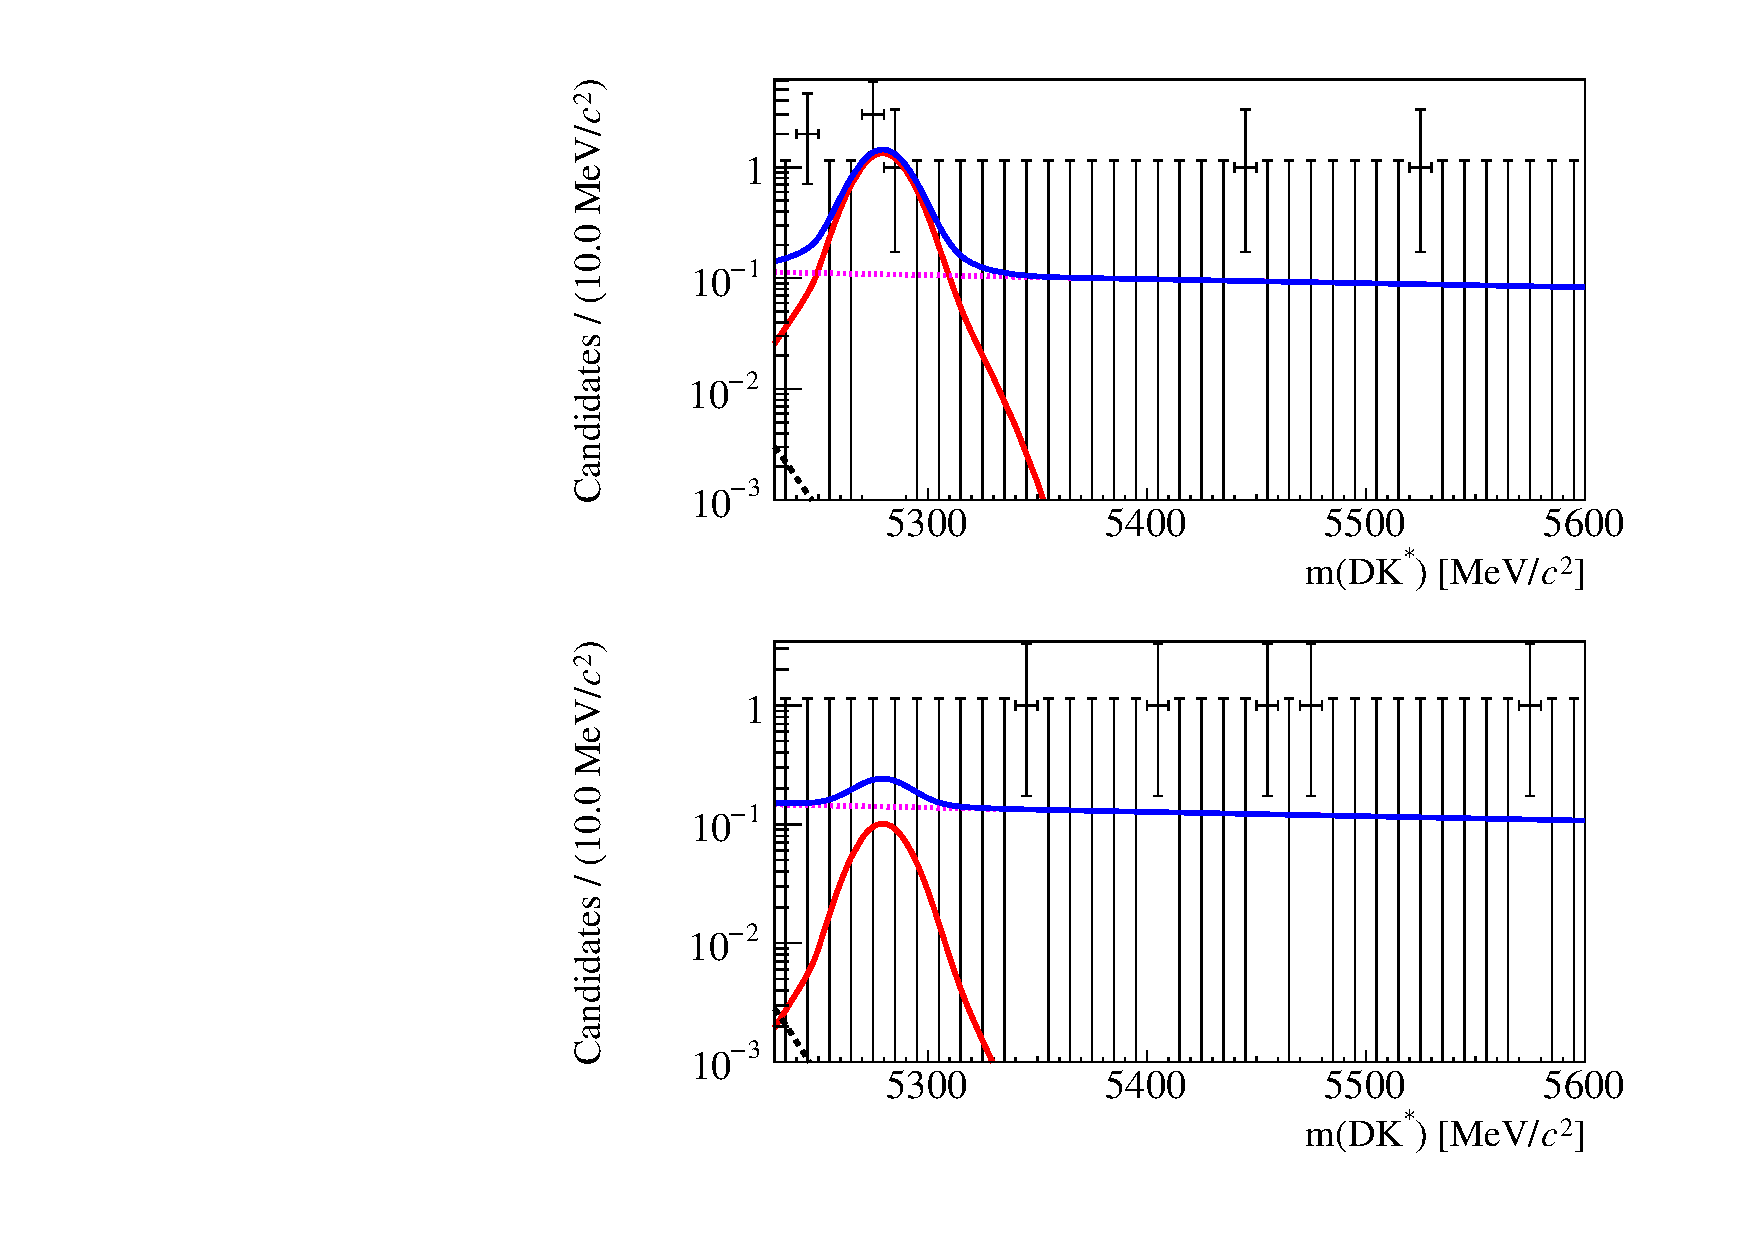
\includegraphics[width=0.25\linewidth]{figures/results/canvaslog_d2pik_DD_run1_log.pdf}}
\caption{Results of the simultaneous fit for Run 1 data for 2-body modes. In each pair the top plot is for \Bp decays and the bottom plot is for \Bm decays.}
\label{datafit2bodyRun1}
\end{sidewaysfigure}

\begin{sidewaysfigure}[h]
\centering
\subfloat[$K\pi\pi\pi$, LL]{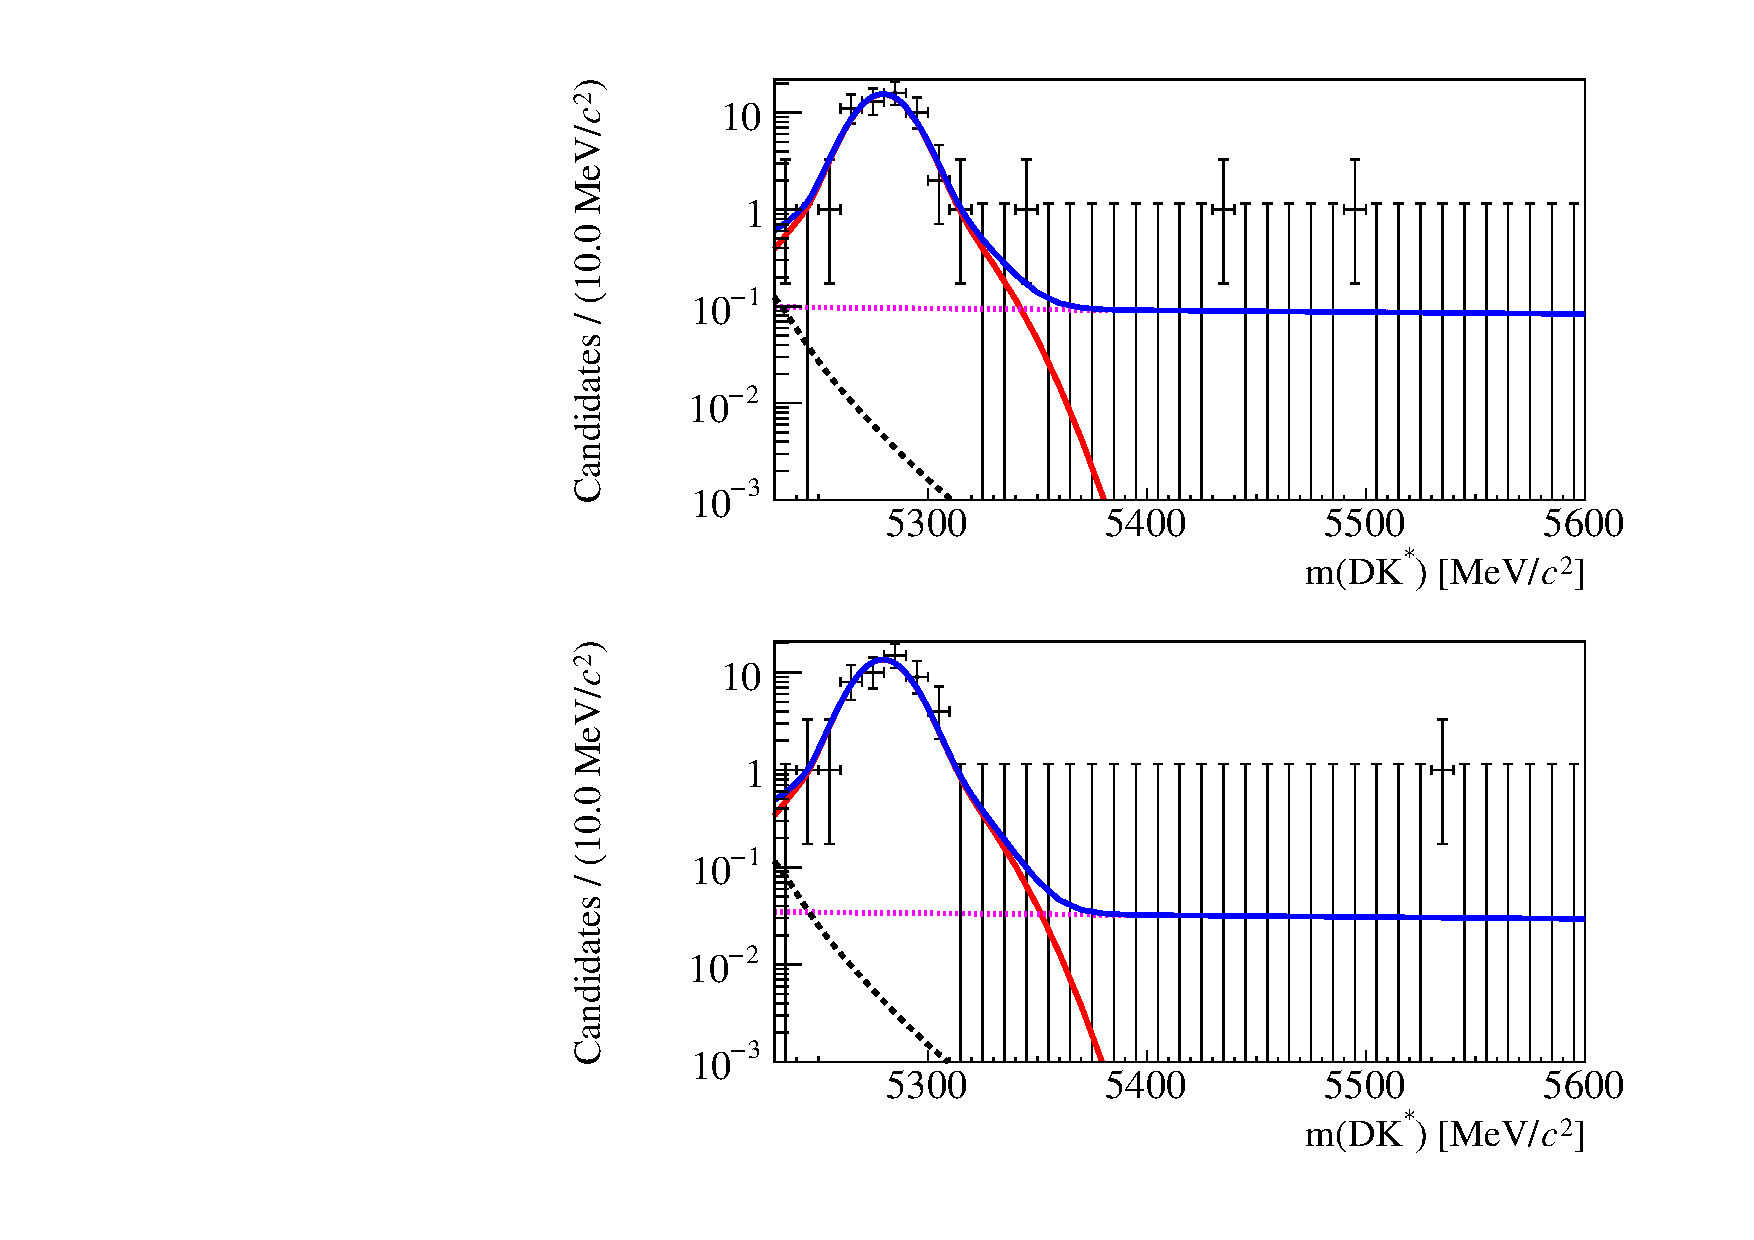
\includegraphics[width=0.3\linewidth]{figures/results/canvaslog_d2kpipipi_LL_run1_log.pdf}}
\hfill
\subfloat[$\pi\pi\pi\pi$, LL]{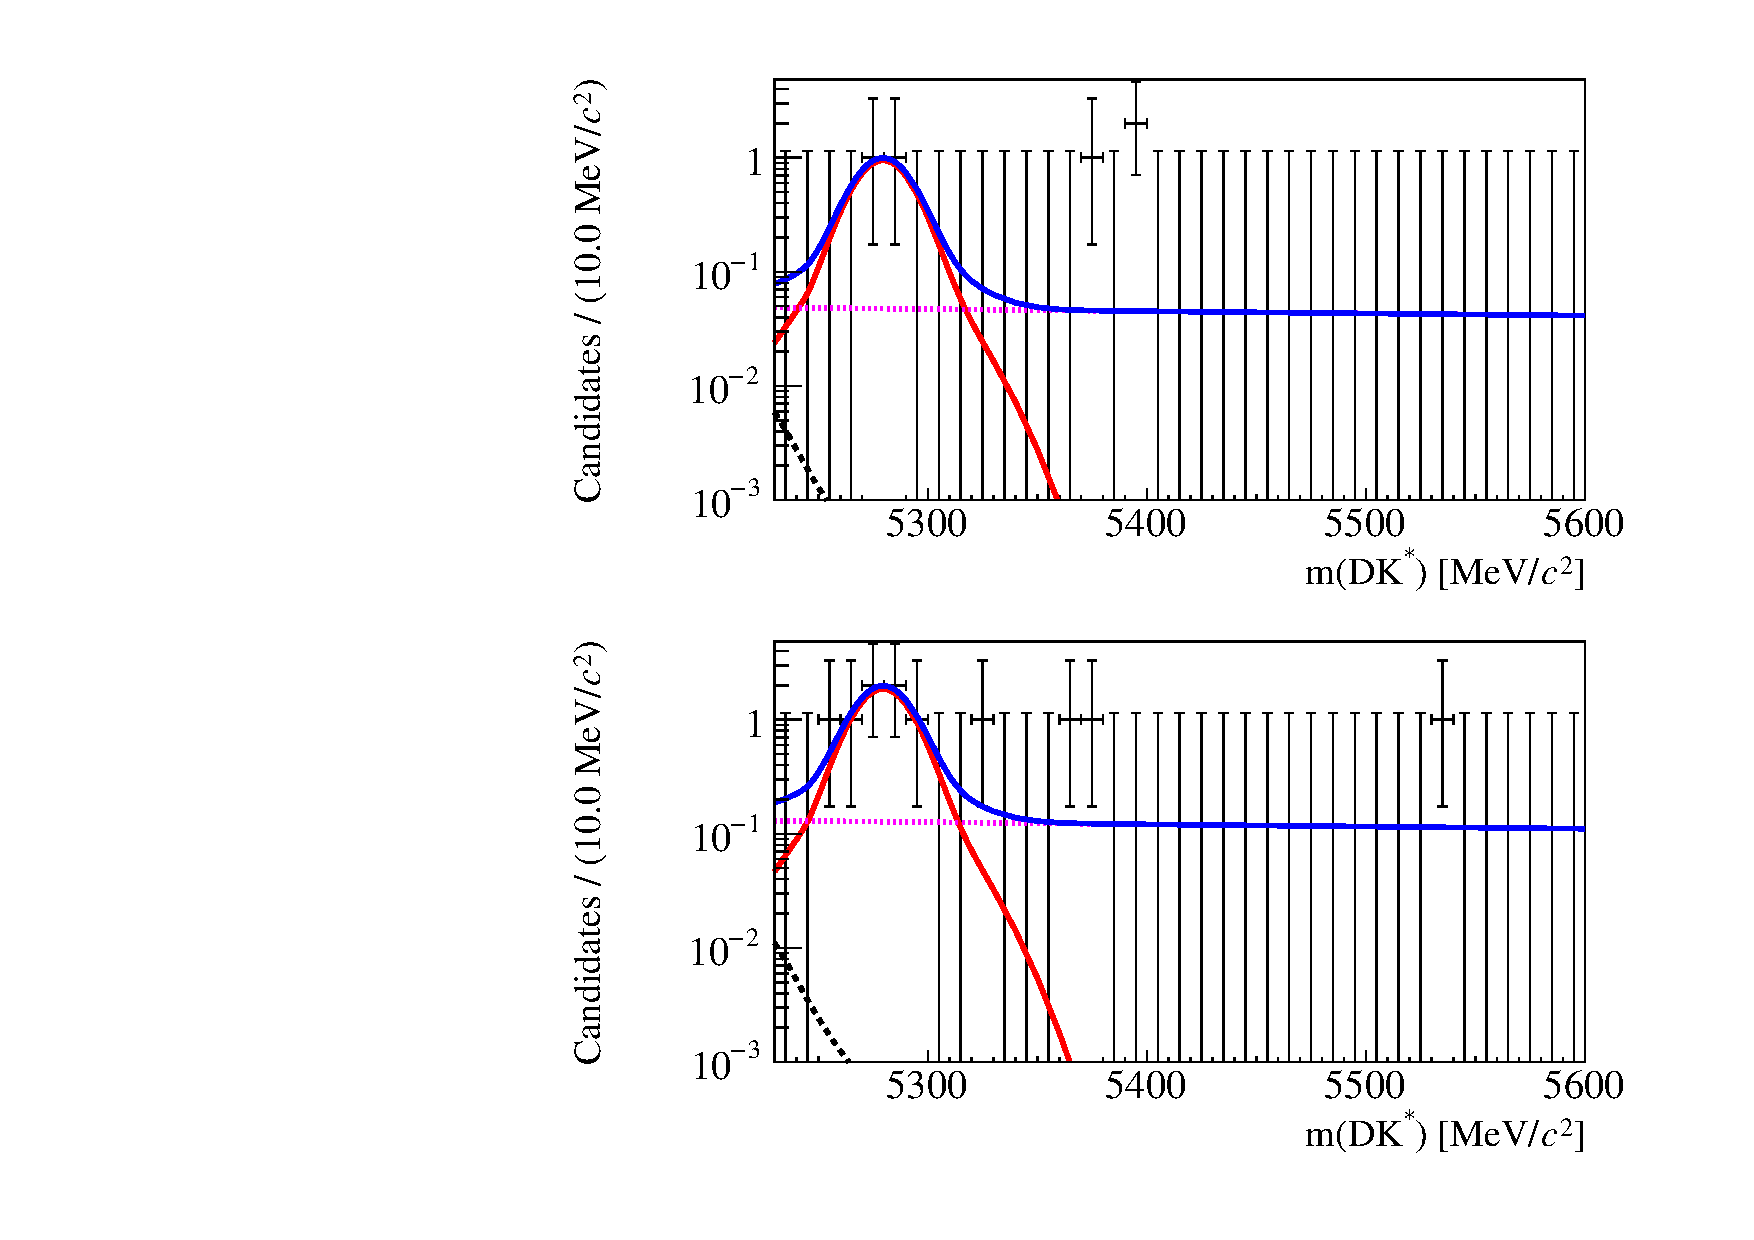
\includegraphics[width=0.3\linewidth]{figures/results/canvaslog_d2pipipipi_LL_run1_log.pdf}}
\hfill
\subfloat[$\pi K\pi\pi$, LL]{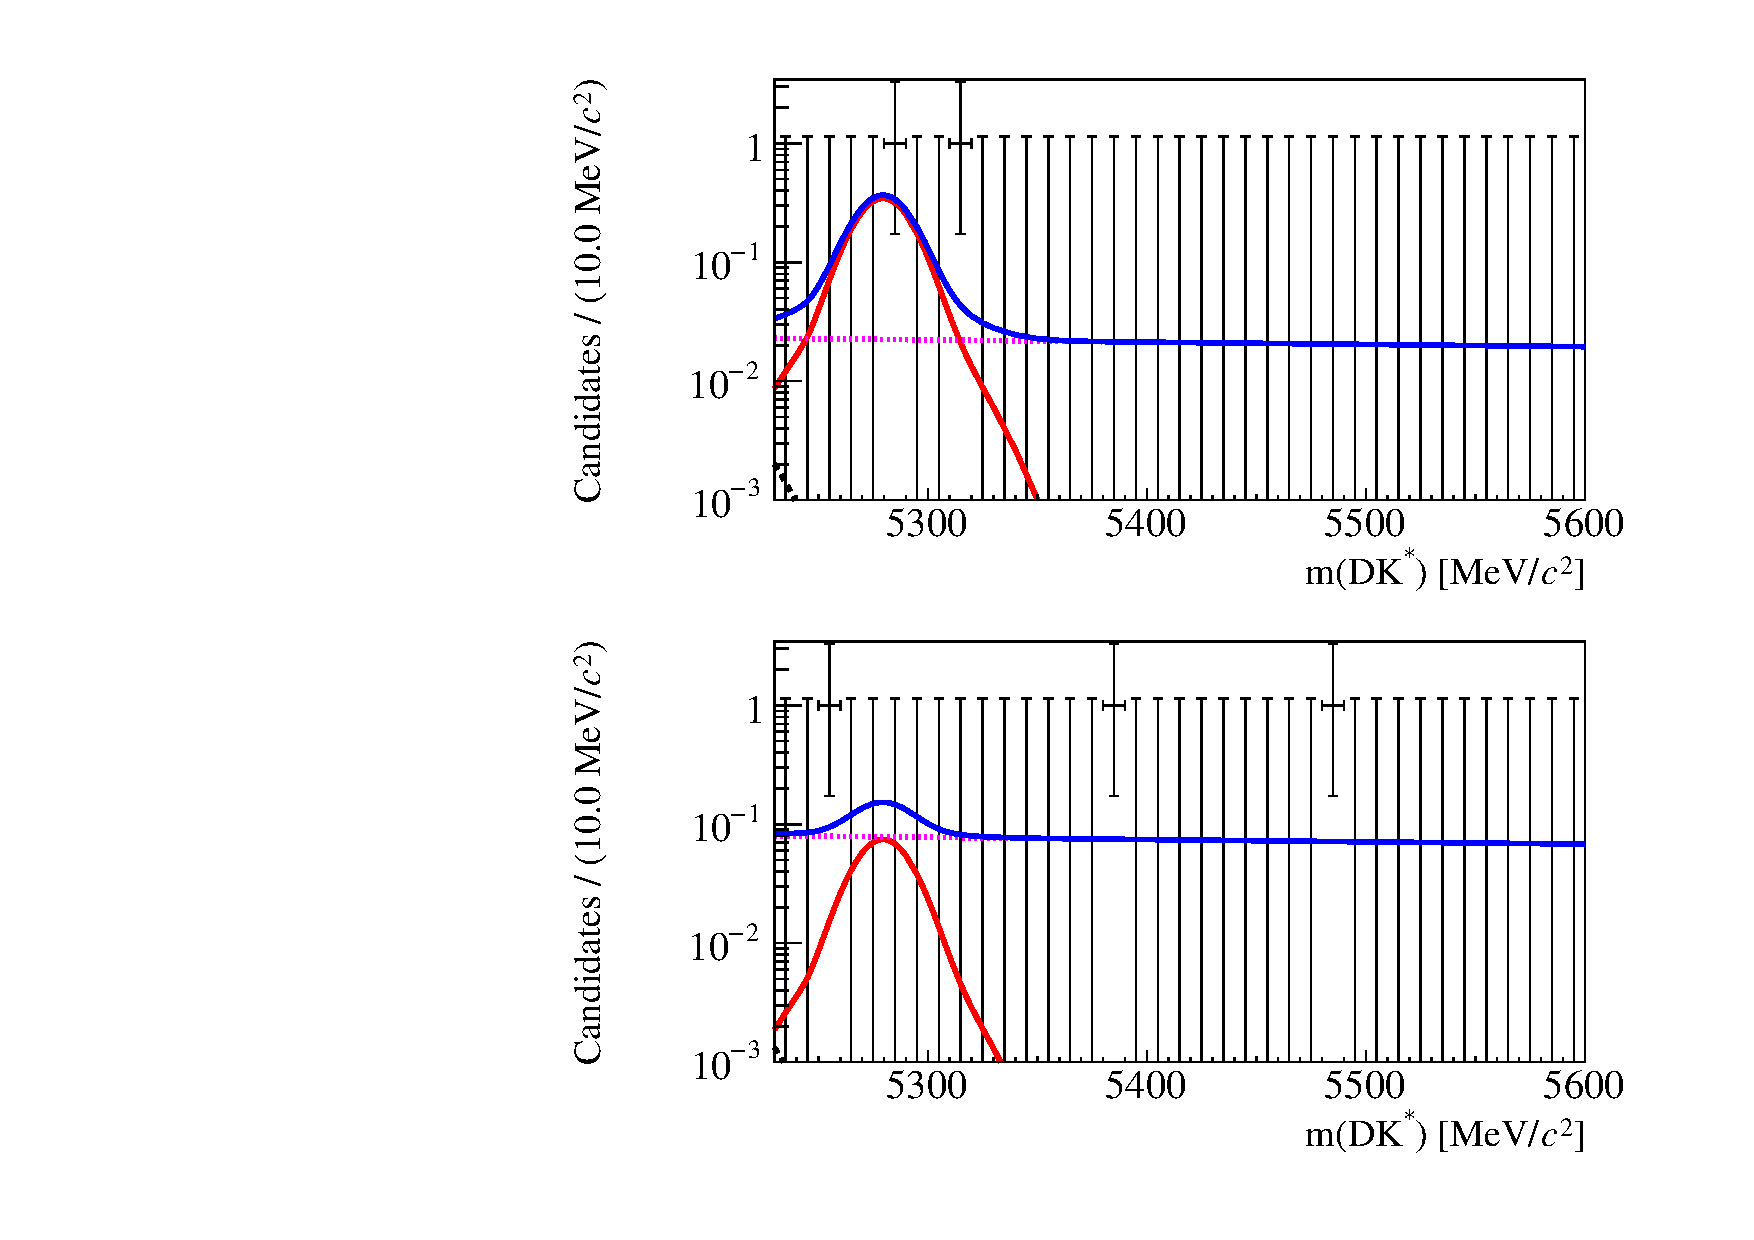
\includegraphics[width=0.3\linewidth]{figures/results/canvaslog_d2pikpipi_LL_run1_log.pdf}}
\hfill
\subfloat[$K\pi\pi\pi$, DD]{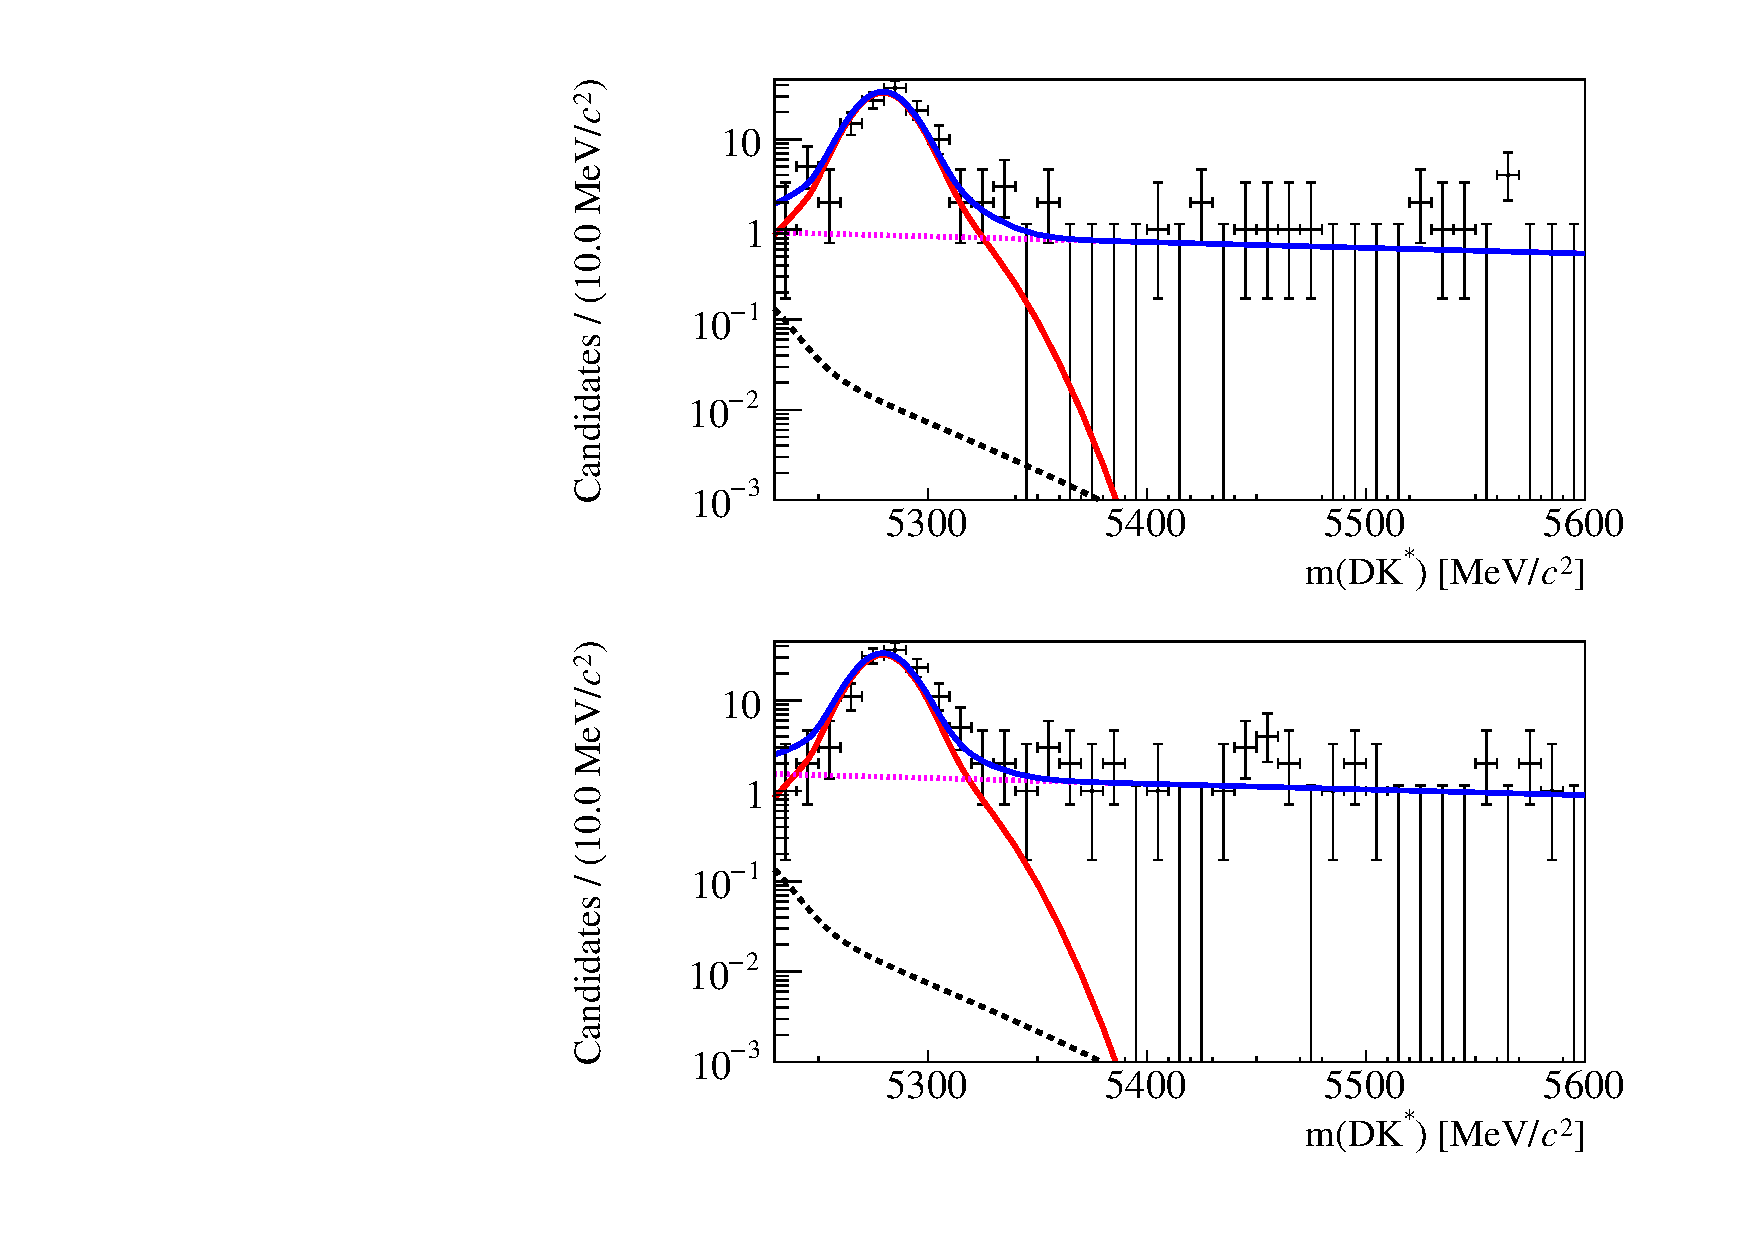
\includegraphics[width=0.3\linewidth]{figures/results/canvaslog_d2kpipipi_DD_run1_log.pdf}}
\hfill
\subfloat[$\pi\pi\pi\pi$, DD]{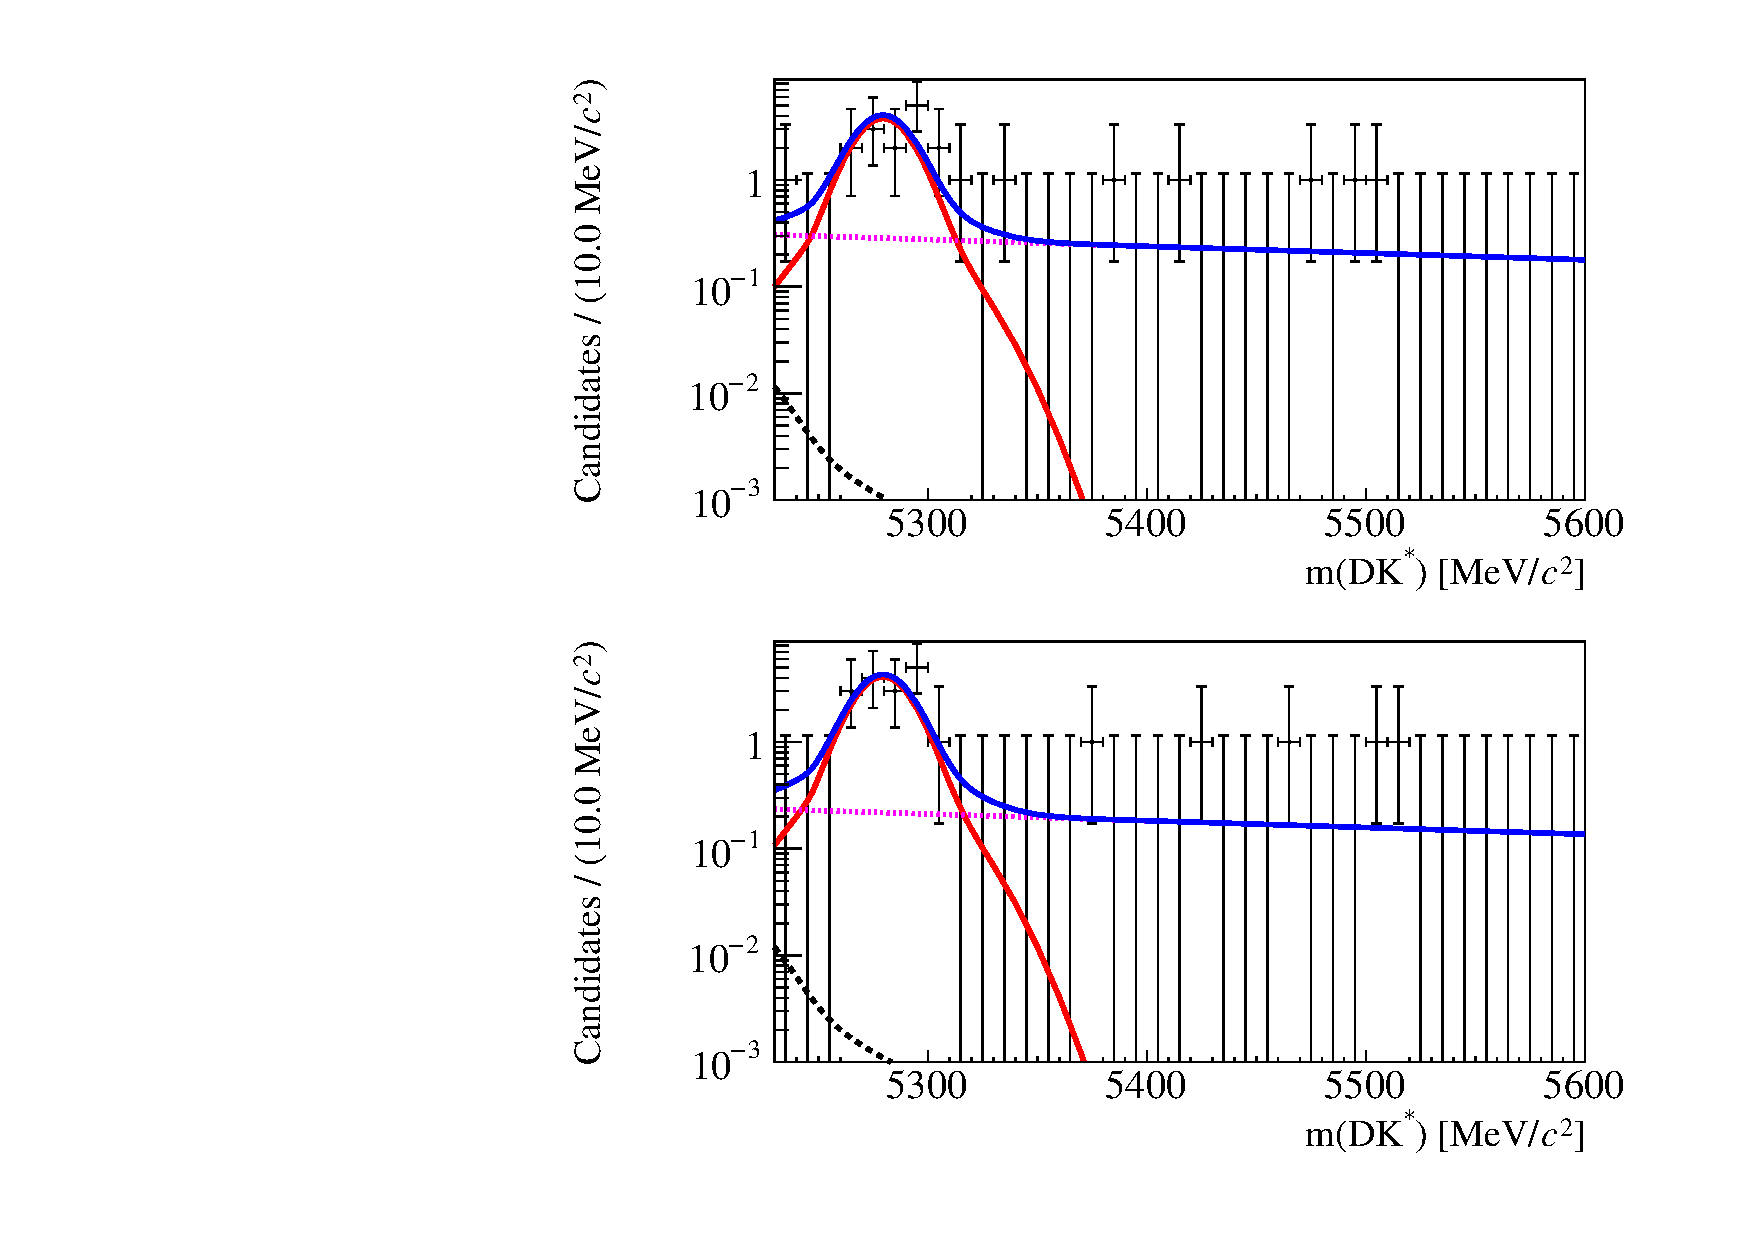
\includegraphics[width=0.3\linewidth]{figures/results/canvaslog_d2pipipipi_DD_run1_log.pdf}}
\hfill
\subfloat[$\pi K\pi\pi$, DD]{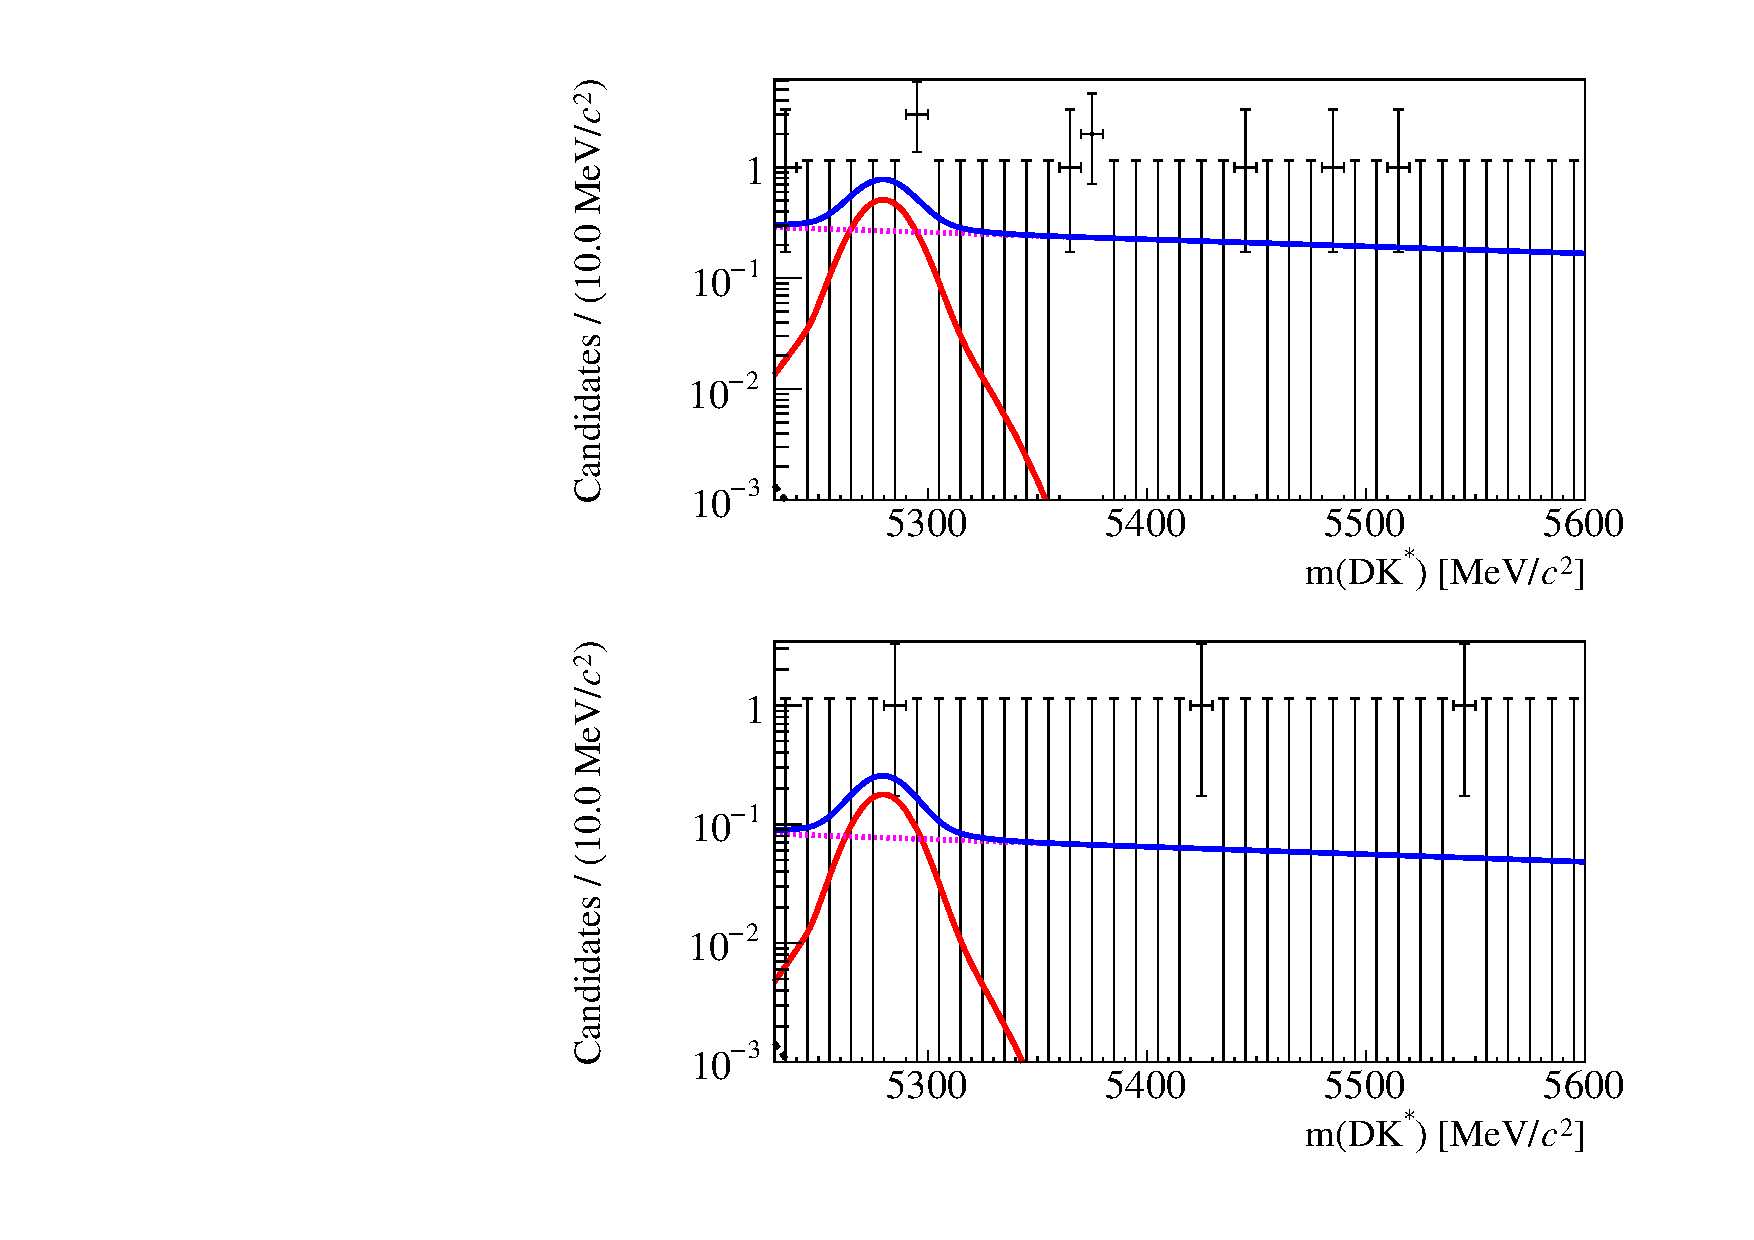
\includegraphics[width=0.3\linewidth]{figures/results/canvaslog_d2pikpipi_DD_run1_log.pdf}}
\caption{Results of the simultaneous fit for Run 1 data for 4-body modes. In each pair the top plot is for \Bp decays and the bottom plot is for \Bm decays.}
\label{datafit4bodyRun1}
\end{sidewaysfigure}

\begin{sidewaysfigure}[h]
\centering
\subfloat[$K\pi$, LL]{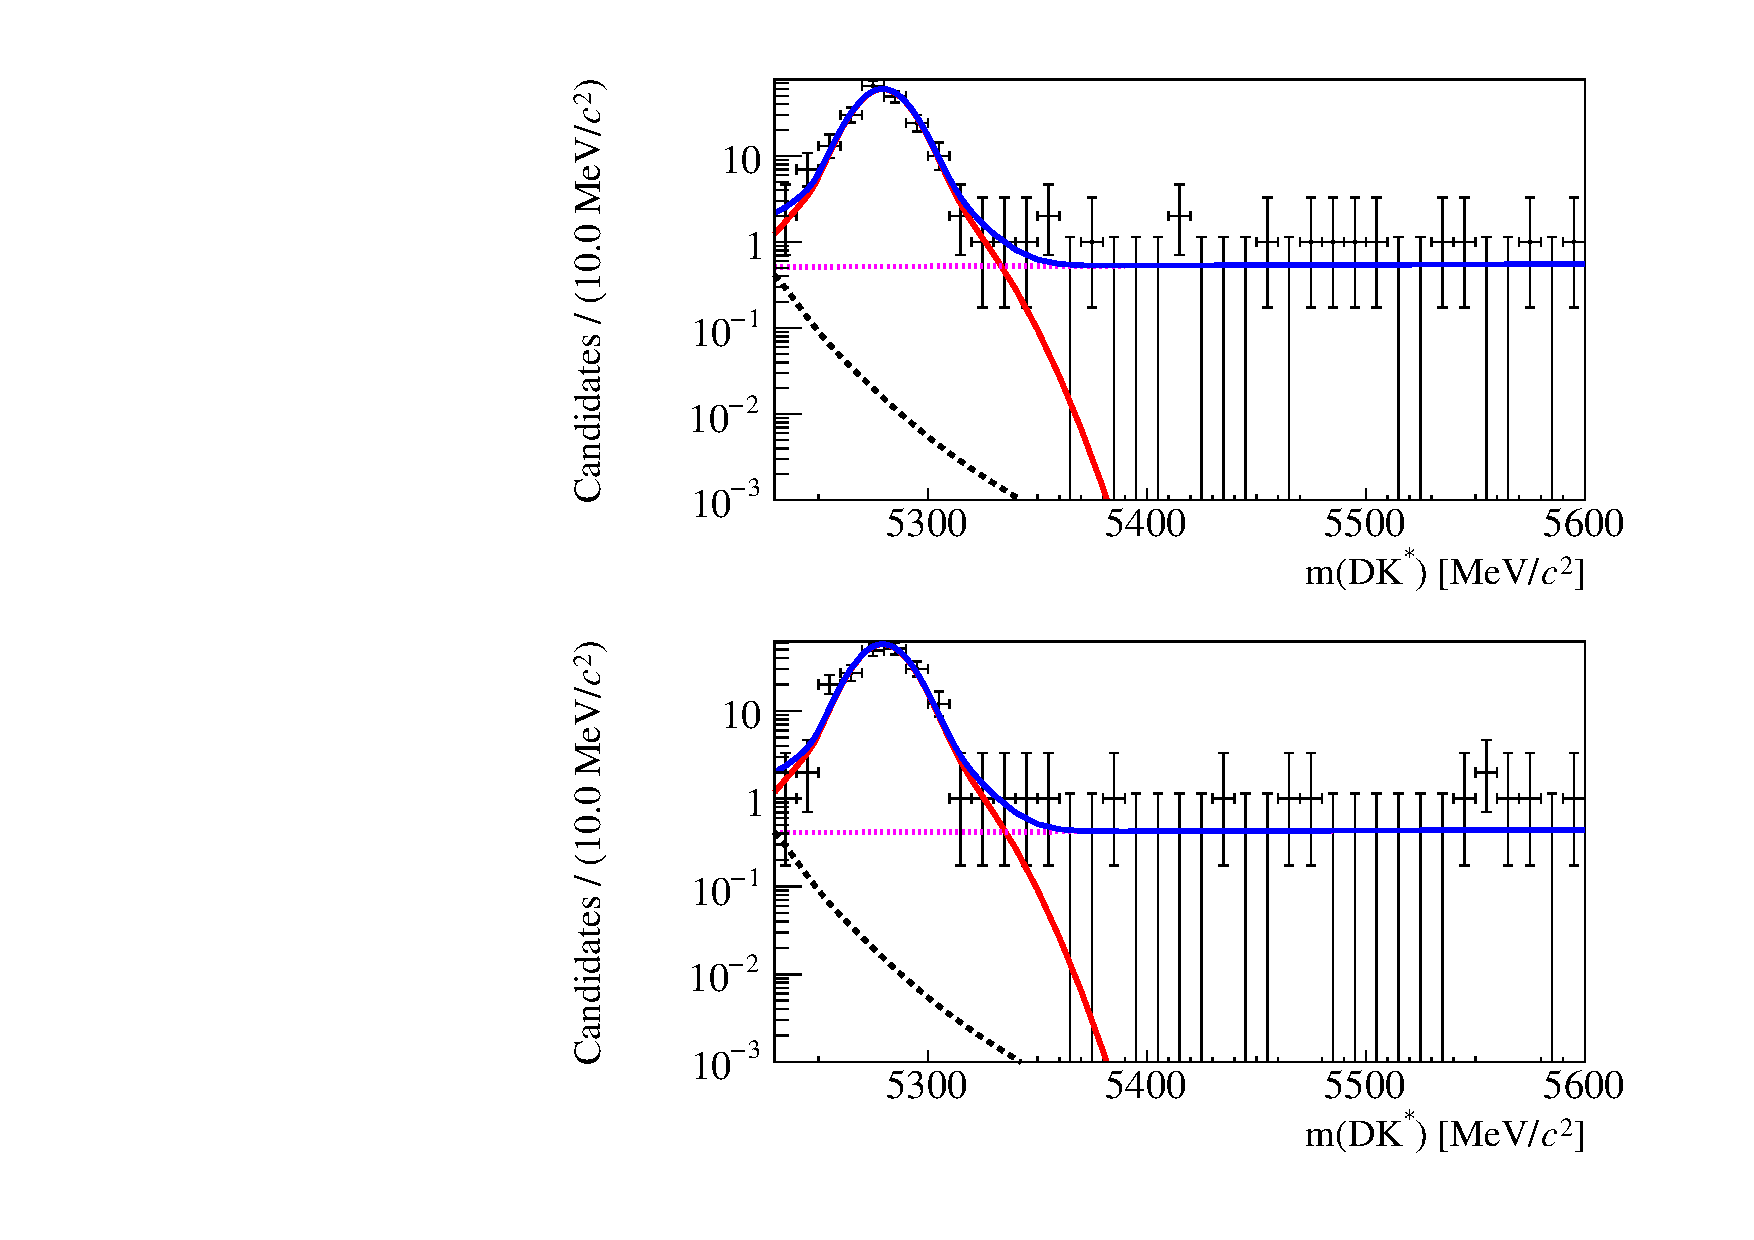
\includegraphics[width=0.25\linewidth]{figures/results/canvaslog_d2kpi_LL_run2_log.pdf}}
\hfill
\subfloat[$KK$, LL]{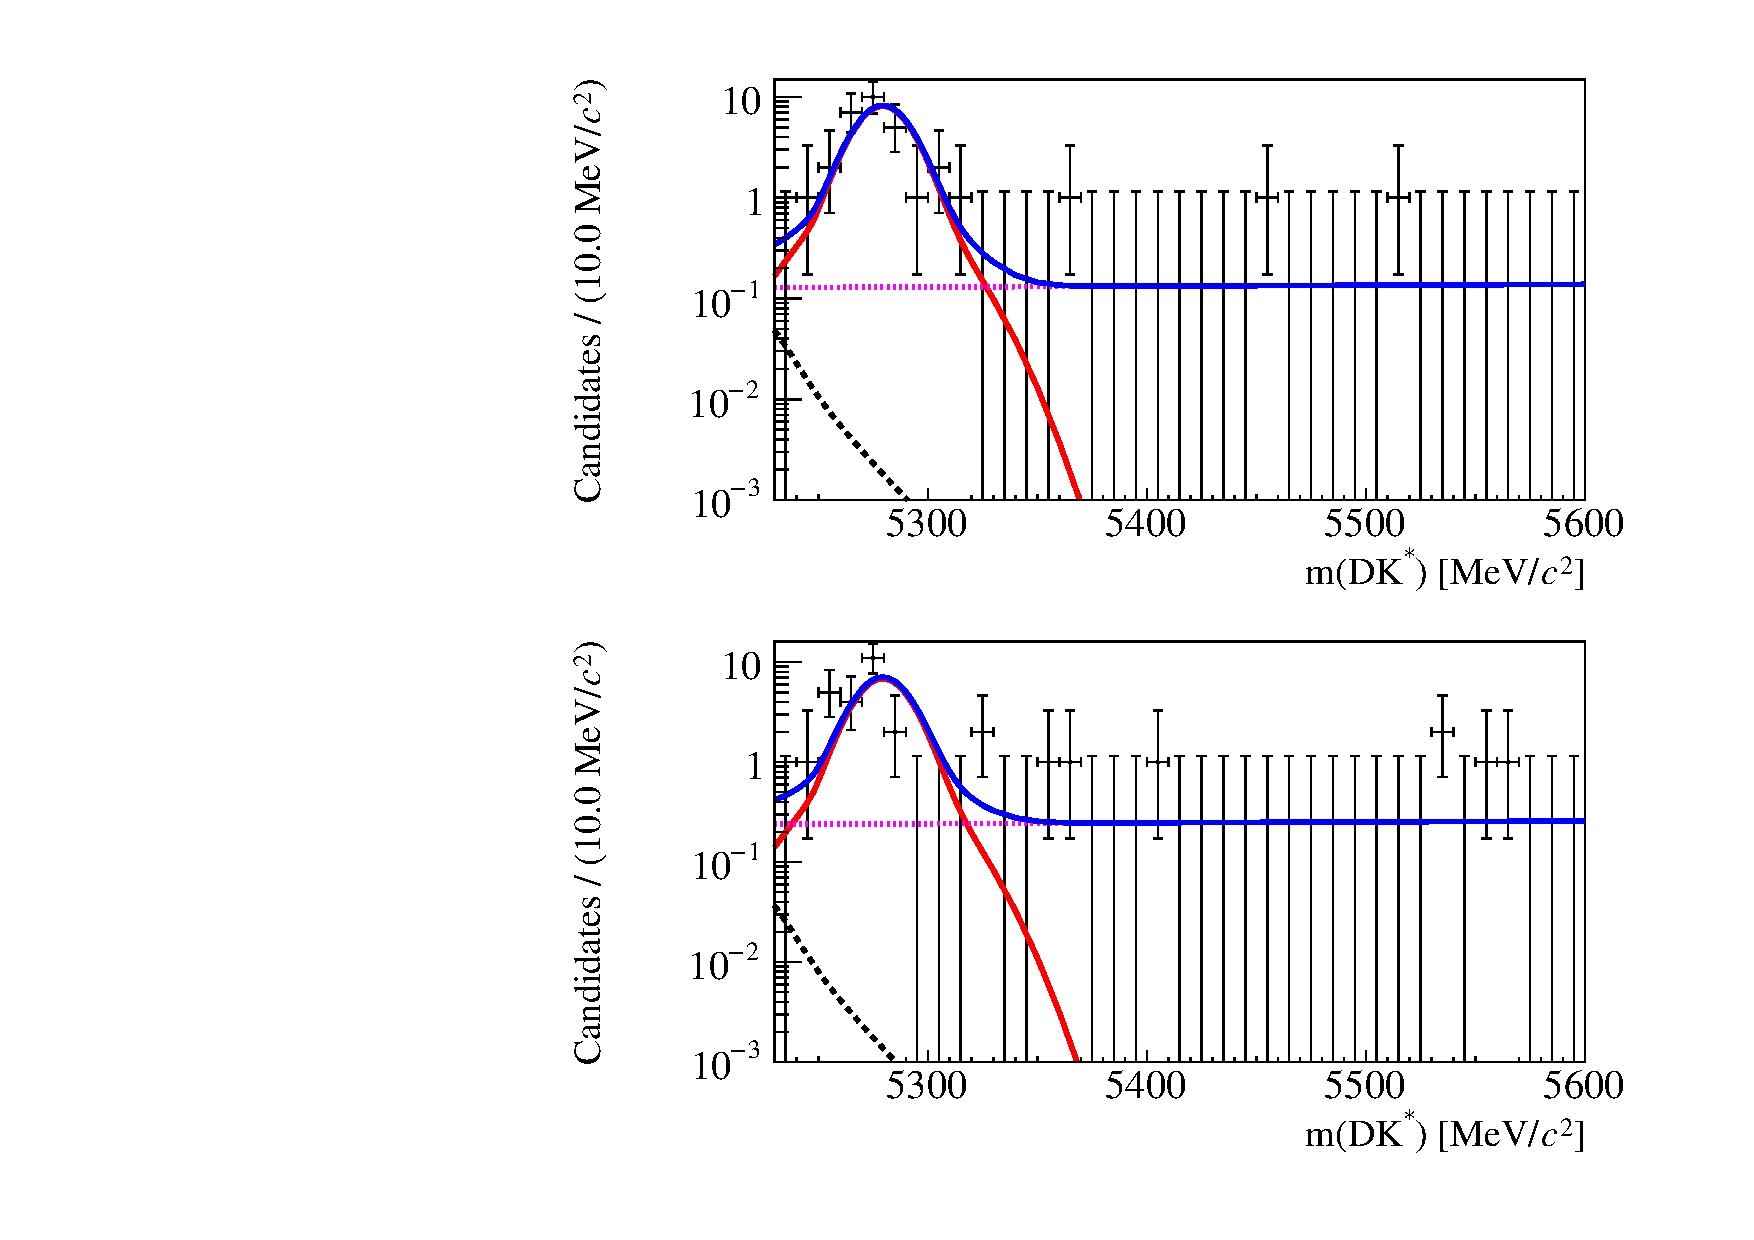
\includegraphics[width=0.25\linewidth]{figures/results/canvaslog_d2kk_LL_run2_log.pdf}}
\hfill
\subfloat[$\pi\pi$, LL]{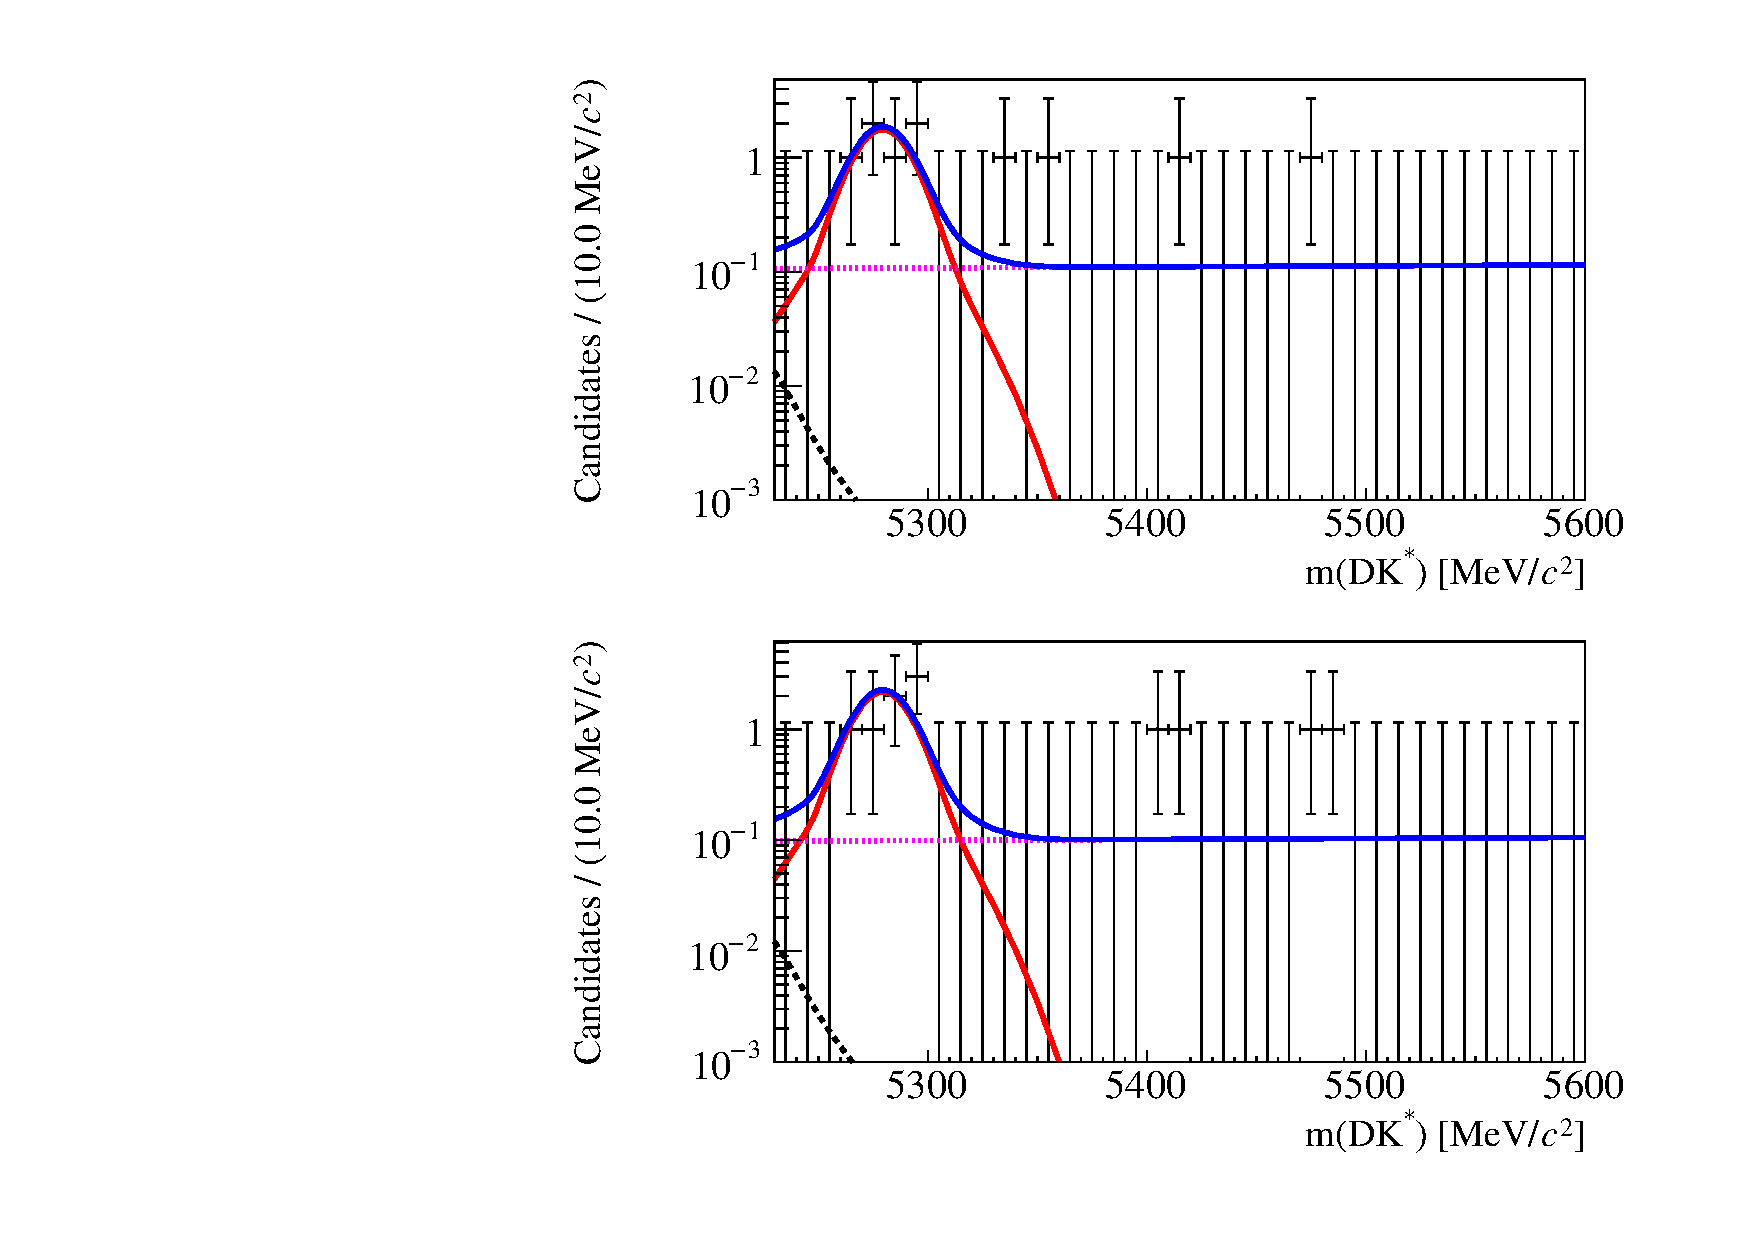
\includegraphics[width=0.25\linewidth]{figures/results/canvaslog_d2pipi_LL_run2_log.pdf}}
\hfill
\subfloat[$\pi K$, LL]{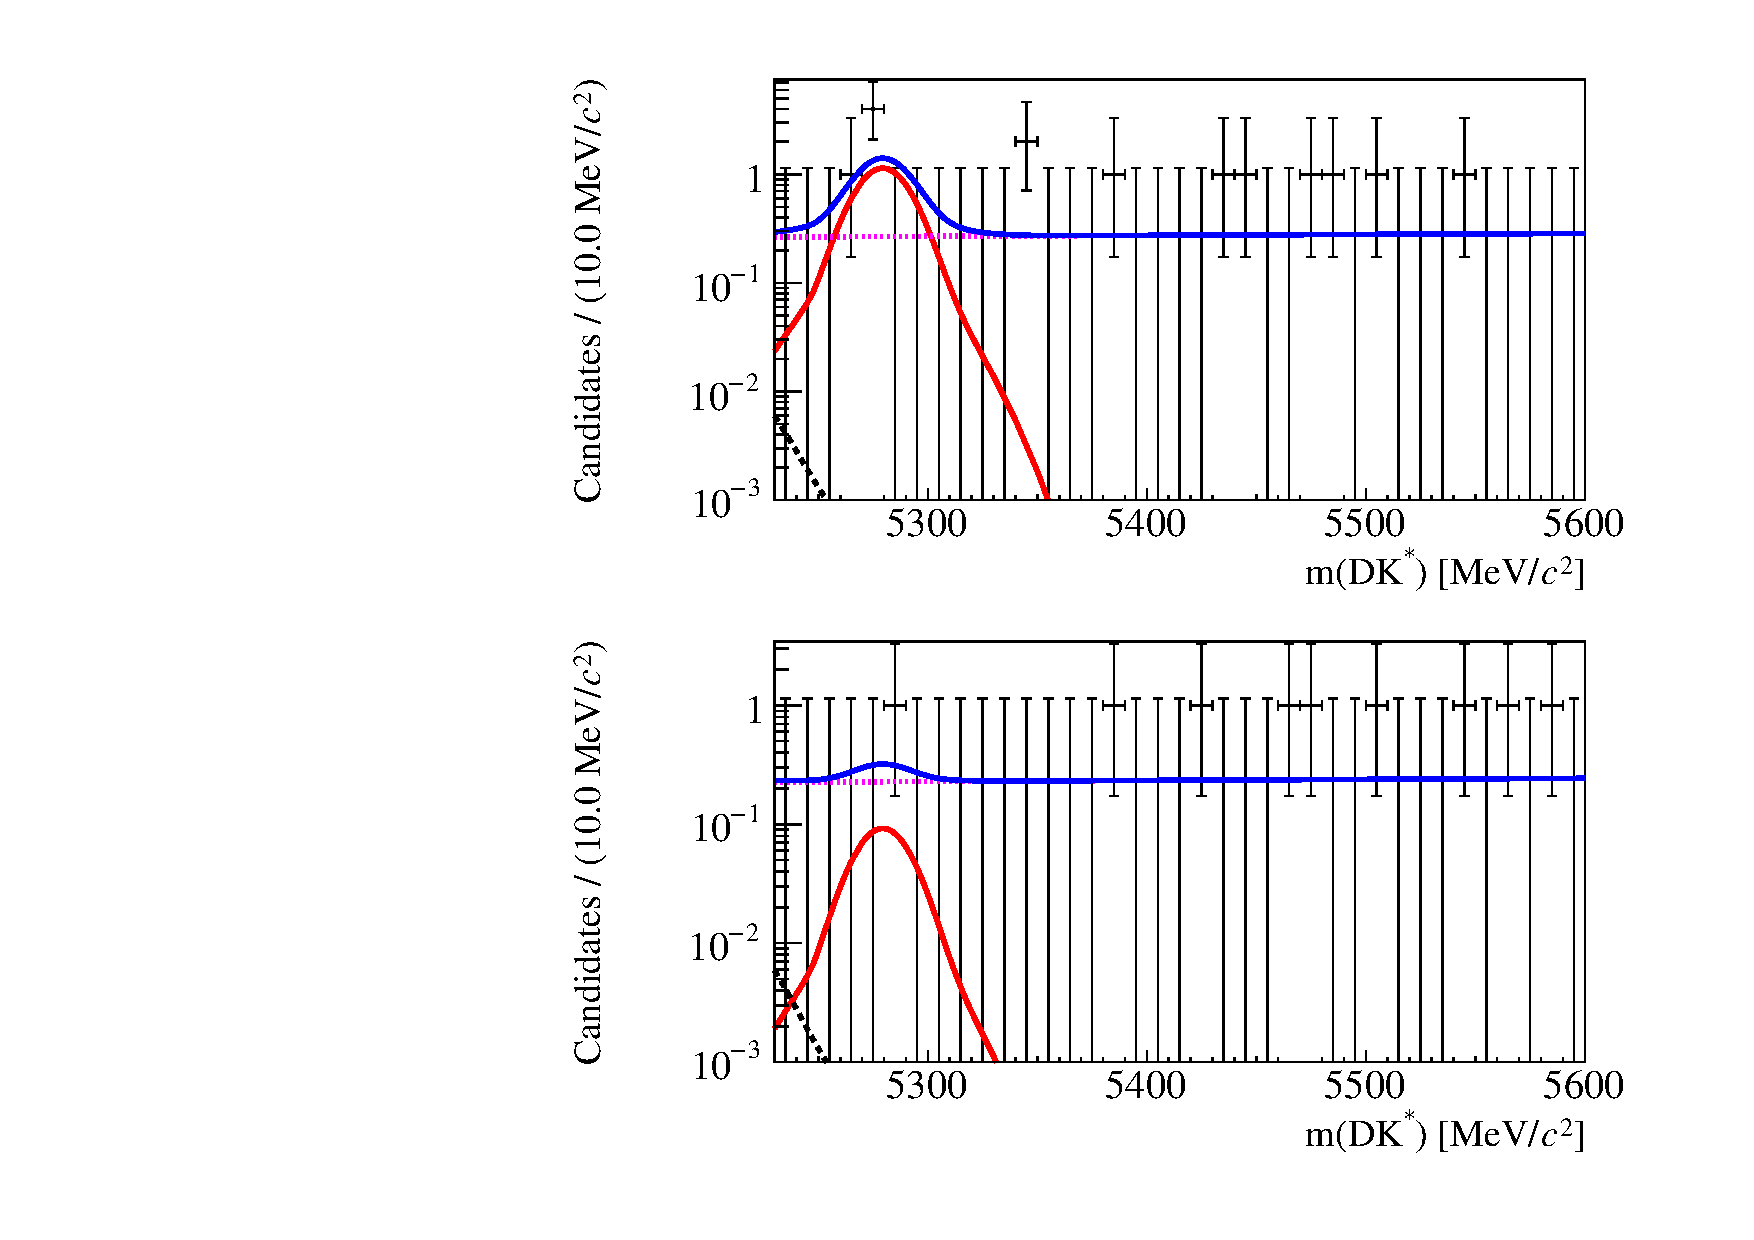
\includegraphics[width=0.25\linewidth]{figures/results/canvaslog_d2pik_LL_run2_log.pdf}}
\hfill
\subfloat[$K\pi$, DD]{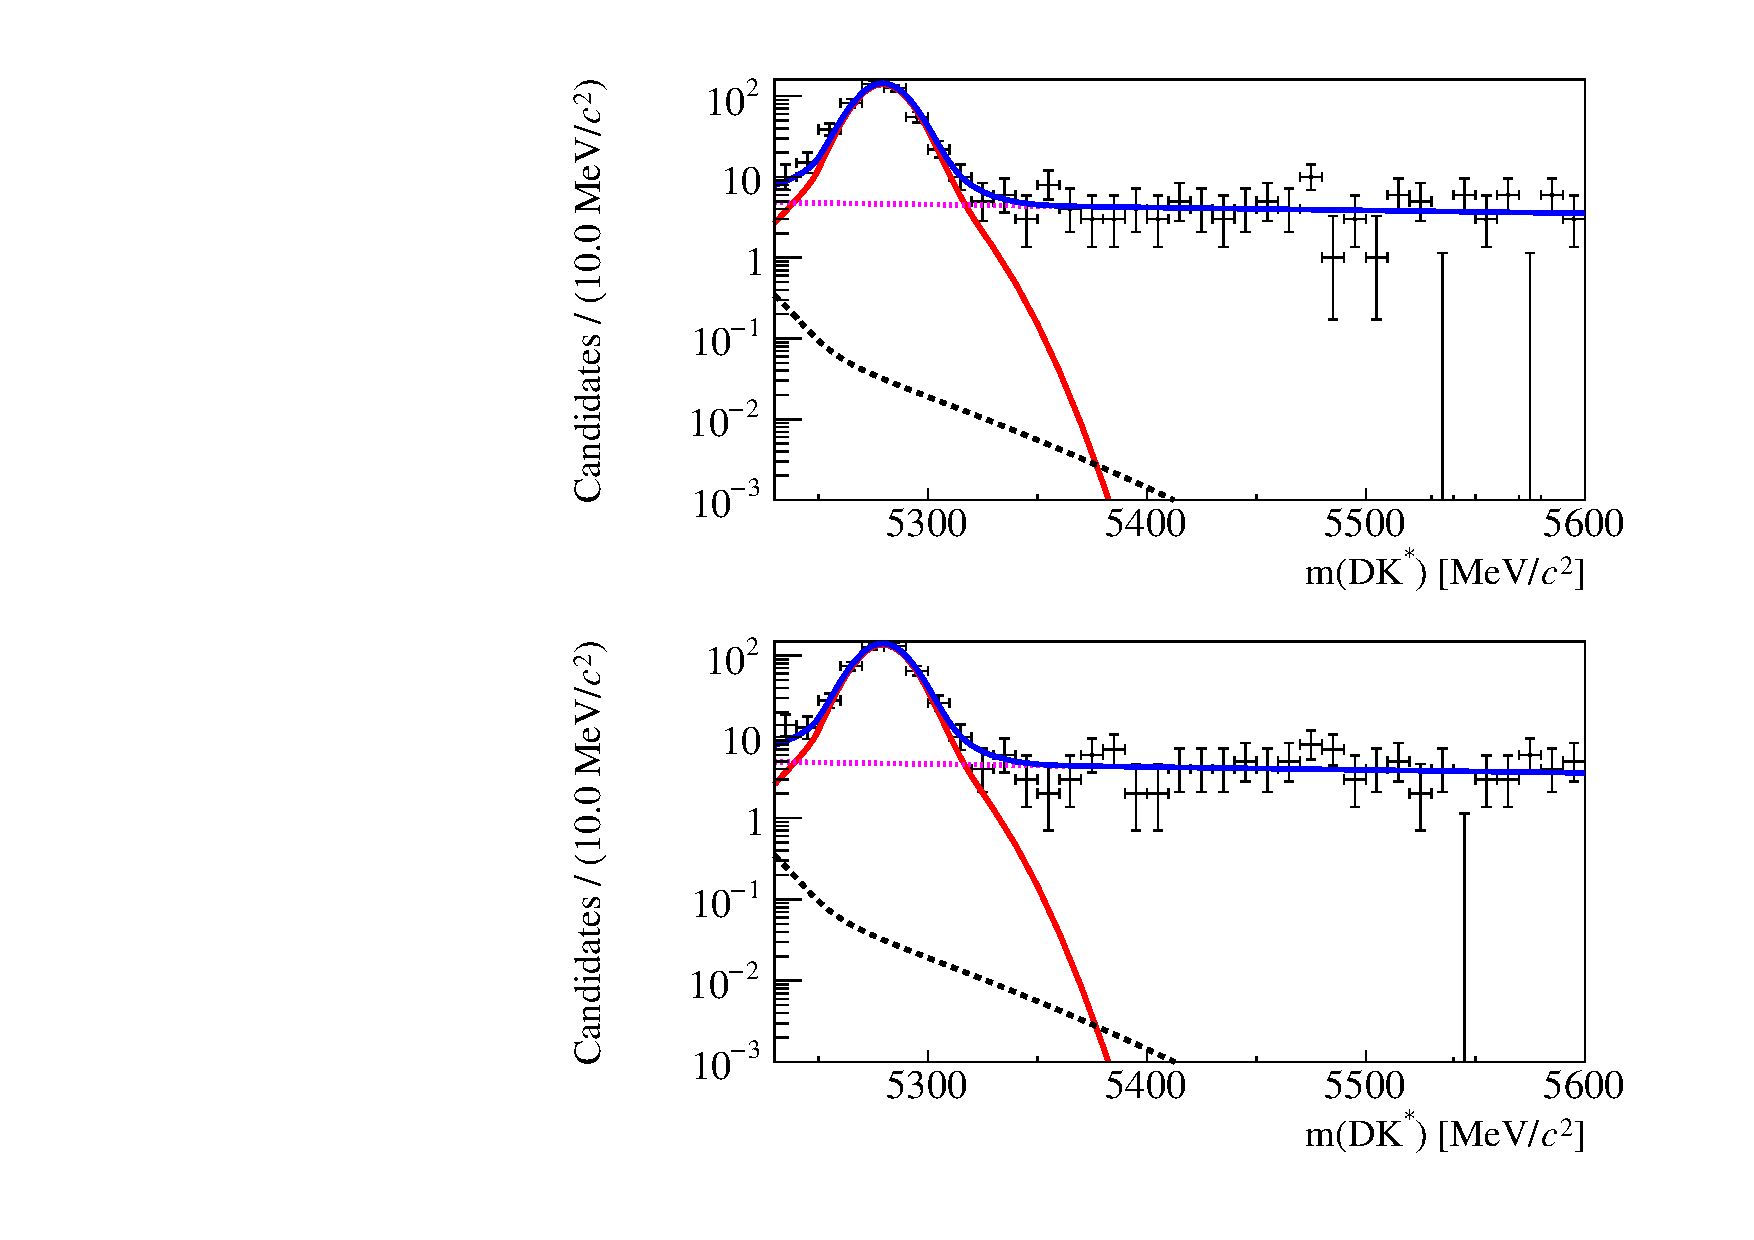
\includegraphics[width=0.25\linewidth]{figures/results/canvaslog_d2kpi_DD_run2_log.pdf}}
\hfill
\subfloat[$KK$, DD]{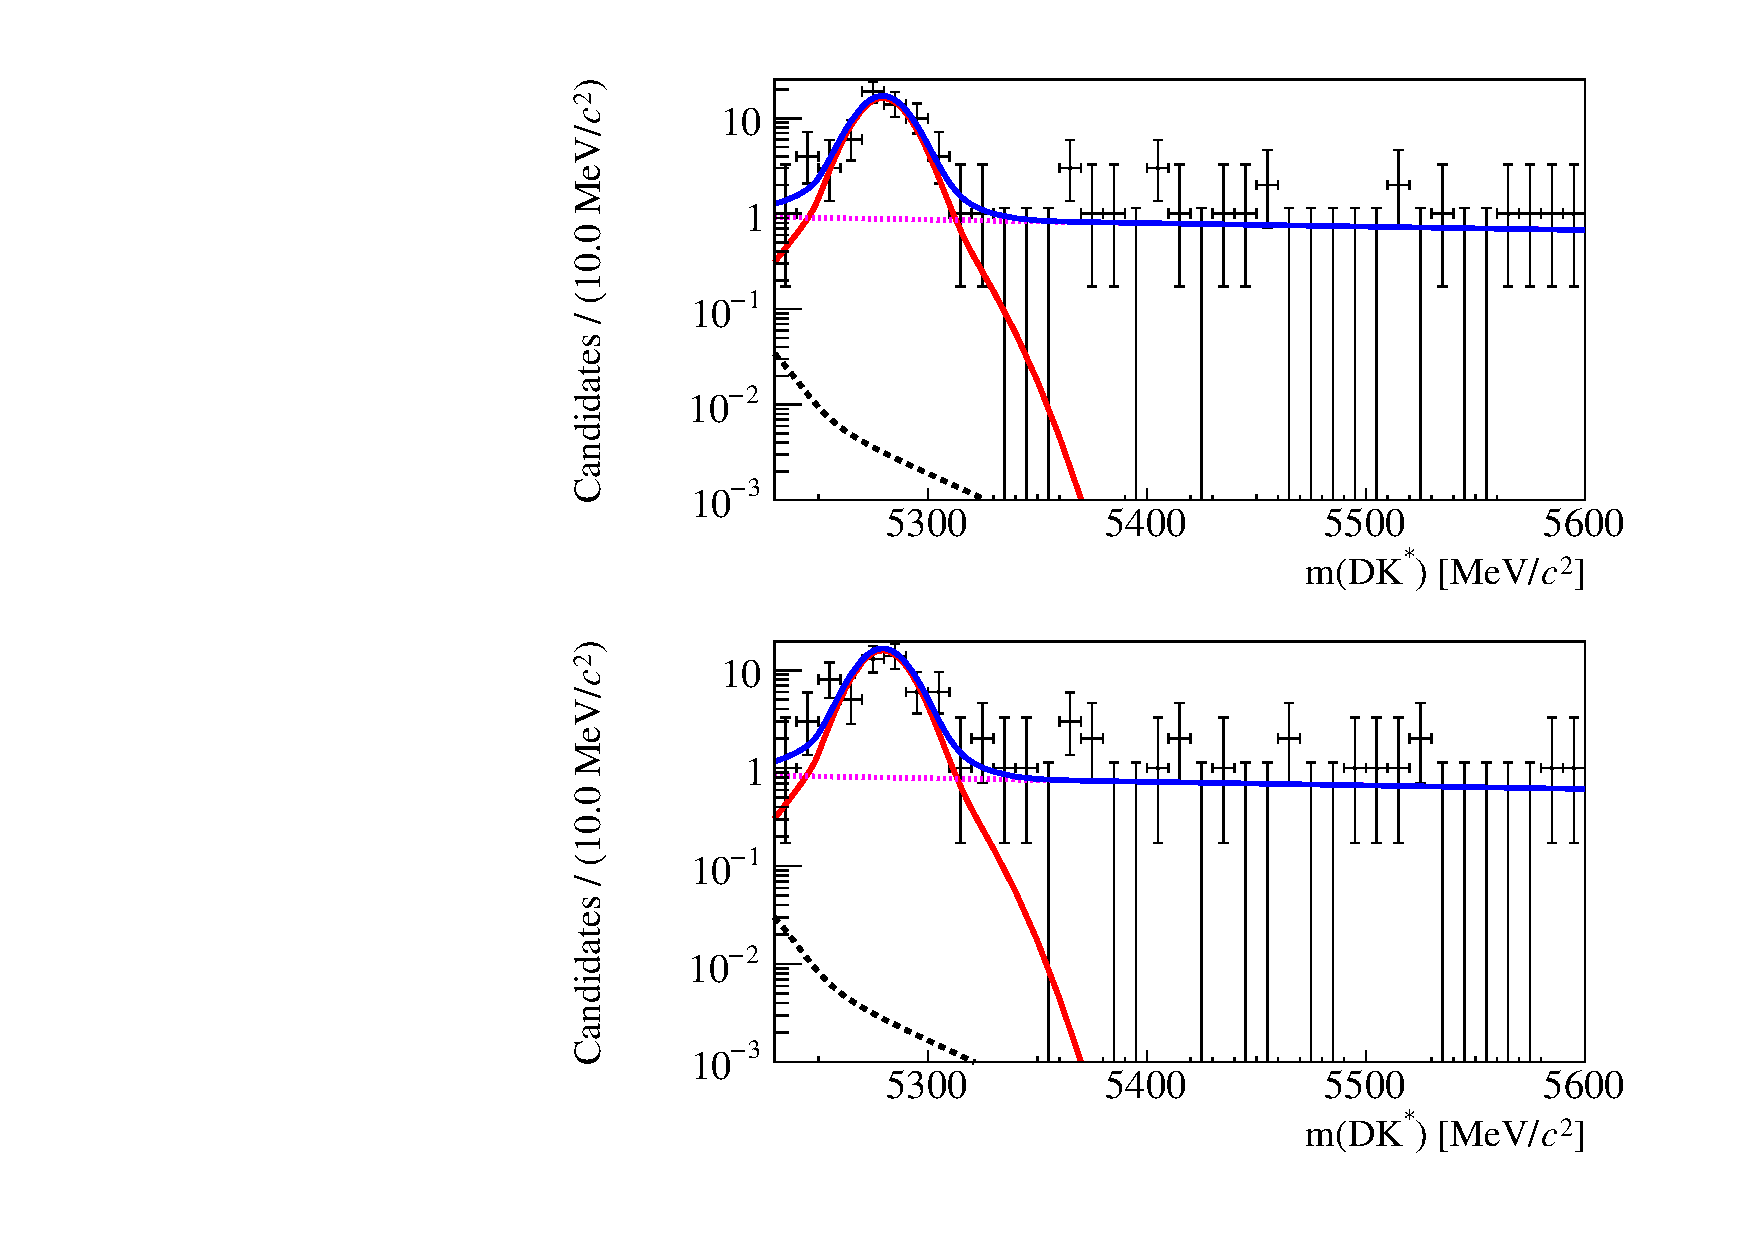
\includegraphics[width=0.25\linewidth]{figures/results/canvaslog_d2kk_DD_run2_log.pdf}}
\hfill
\subfloat[$\pi\pi$, DD]{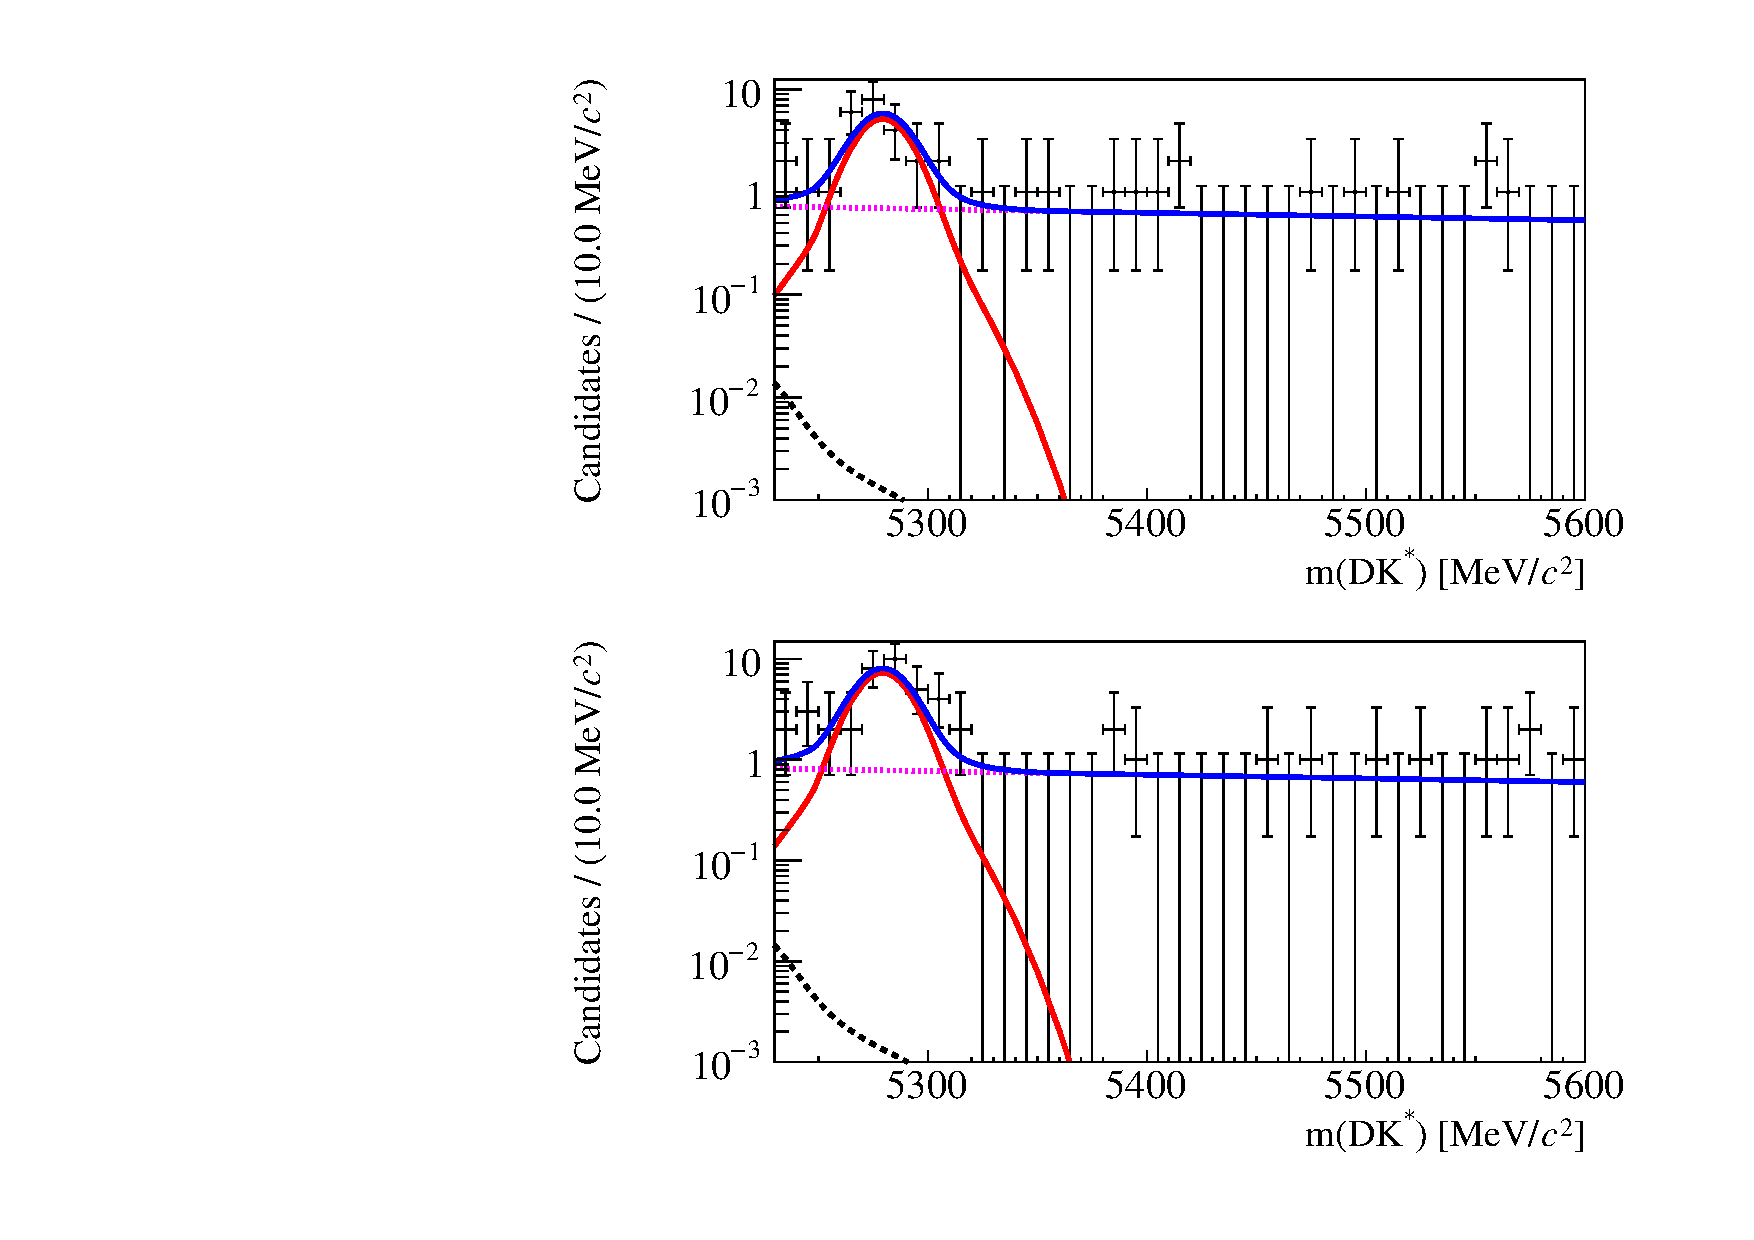
\includegraphics[width=0.25\linewidth]{figures/results/canvaslog_d2pipi_DD_run2_log.pdf}}
\hfill
\subfloat[$\pi K$, DD]{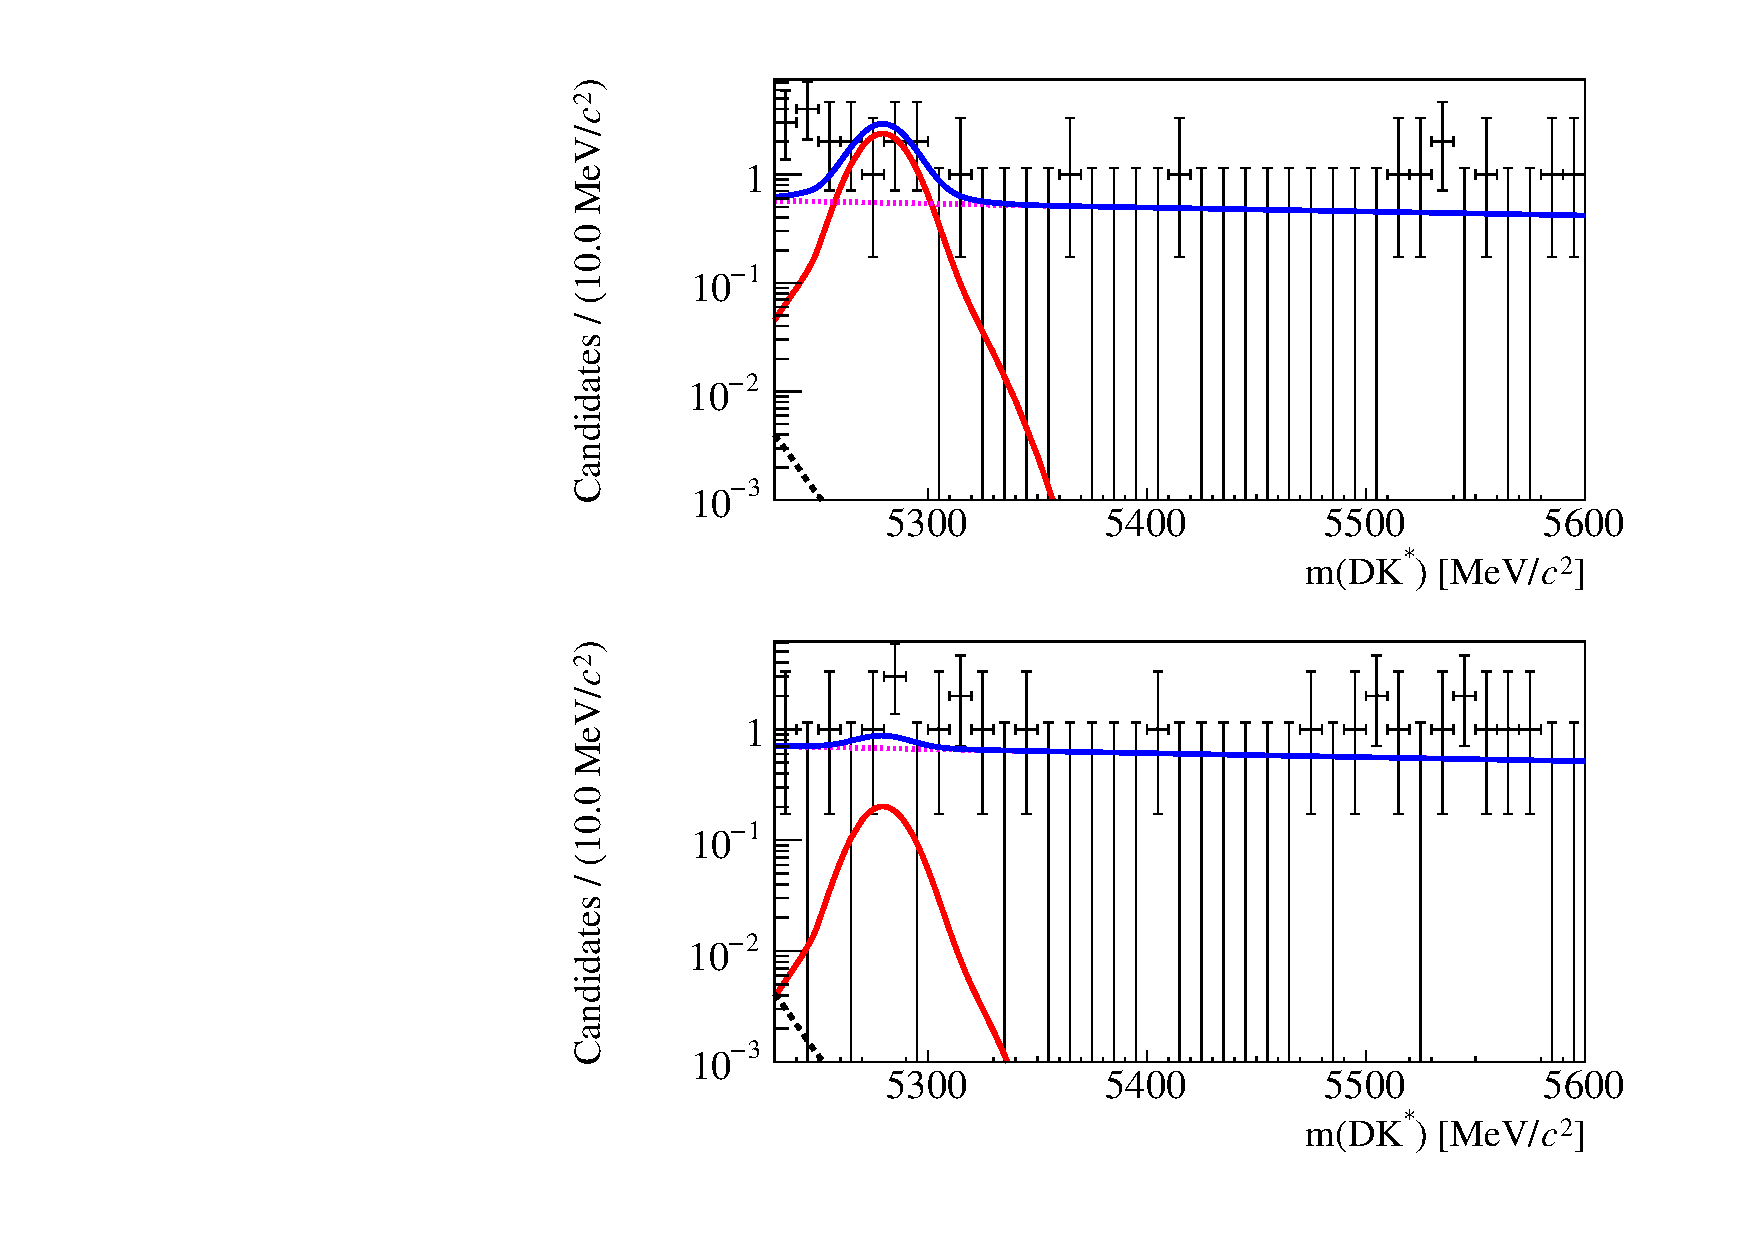
\includegraphics[width=0.25\linewidth]{figures/results/canvaslog_d2pik_DD_run2_log.pdf}}
\caption{Results of the simultaneous fit for Run 1 data for 2-body modes. In each pair the top plot is for \Bp decays and the bottom plot is for \Bm decays.}
\label{datafit2bodyRun2}
\end{sidewaysfigure}

\begin{sidewaysfigure}[h]
\centering
\subfloat[$K\pi\pi\pi$, LL]{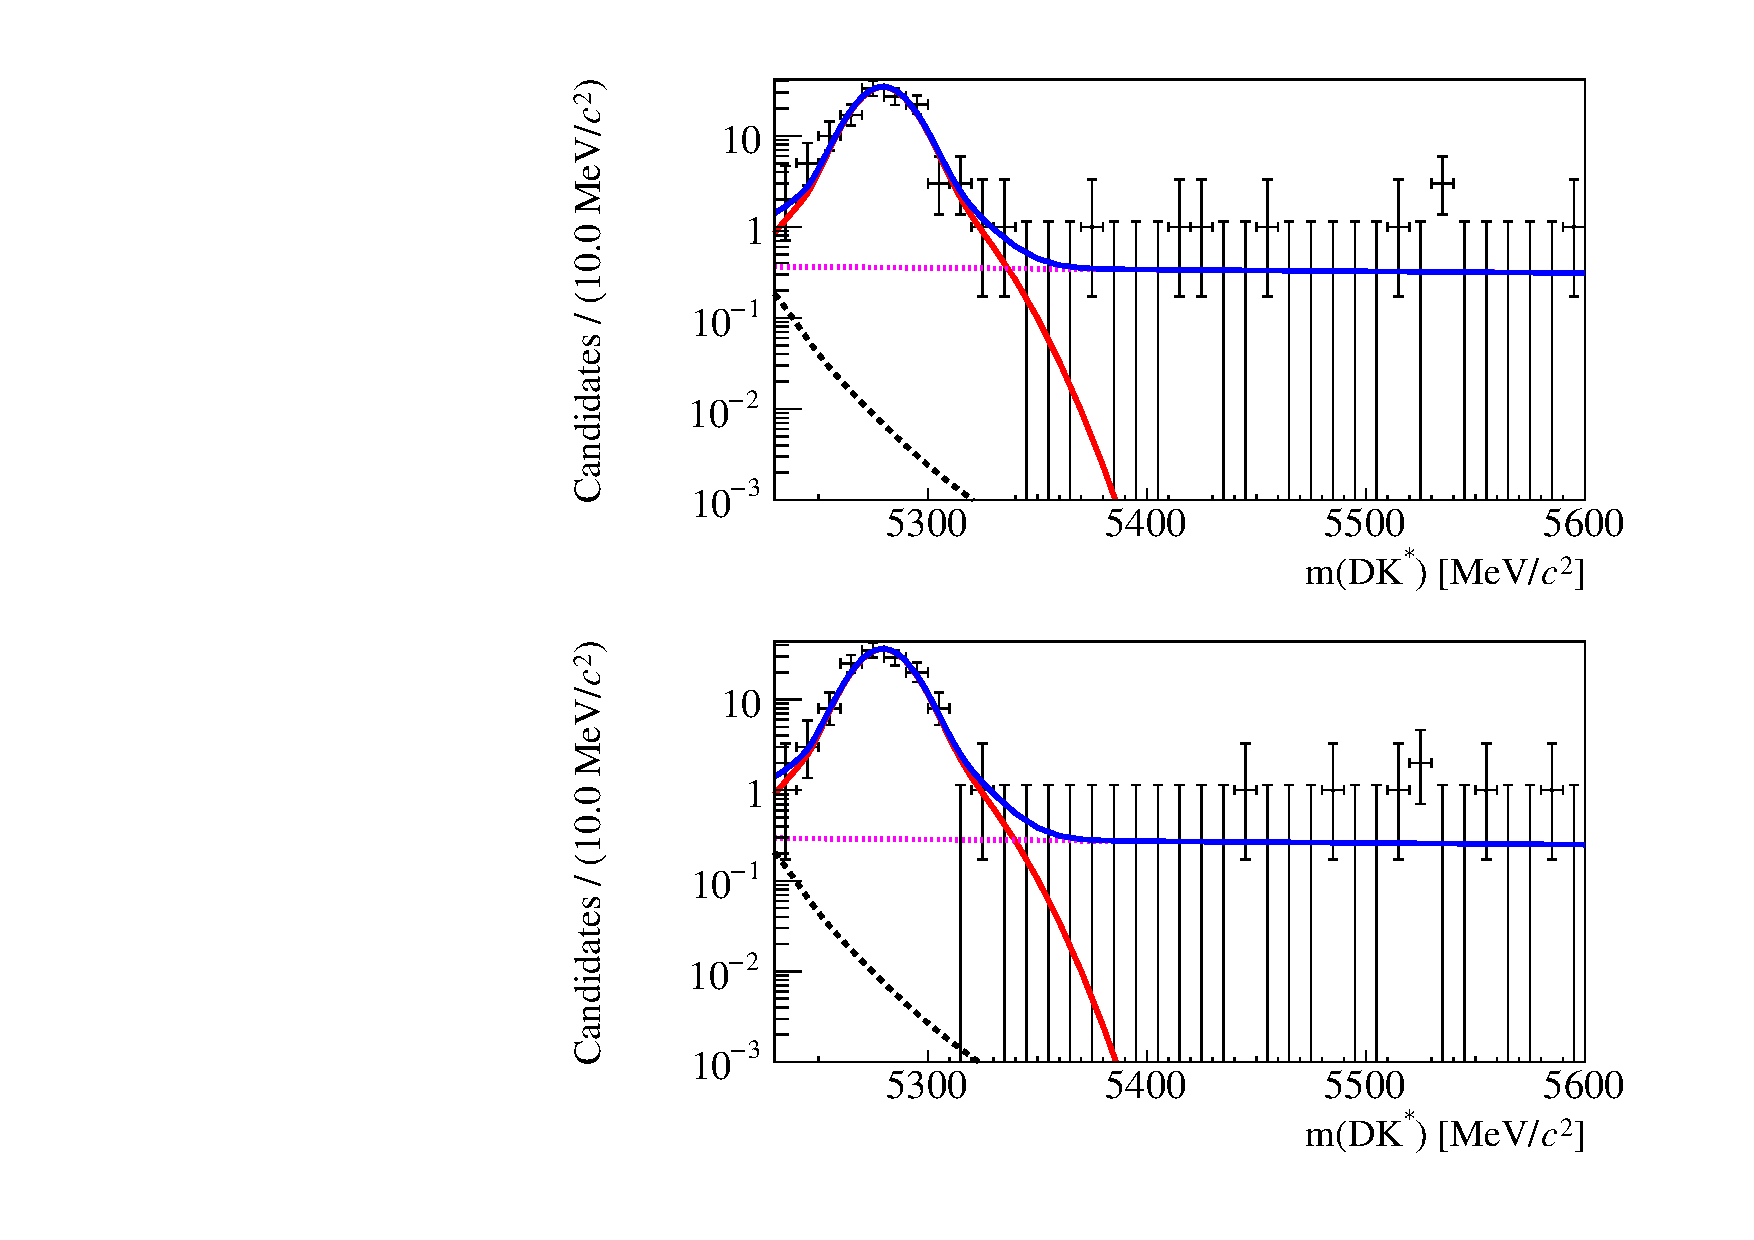
\includegraphics[width=0.3\linewidth]{figures/results/canvaslog_d2kpipipi_LL_run2_log.pdf}}
\hfill
\subfloat[$\pi\pi\pi\pi$, LL]{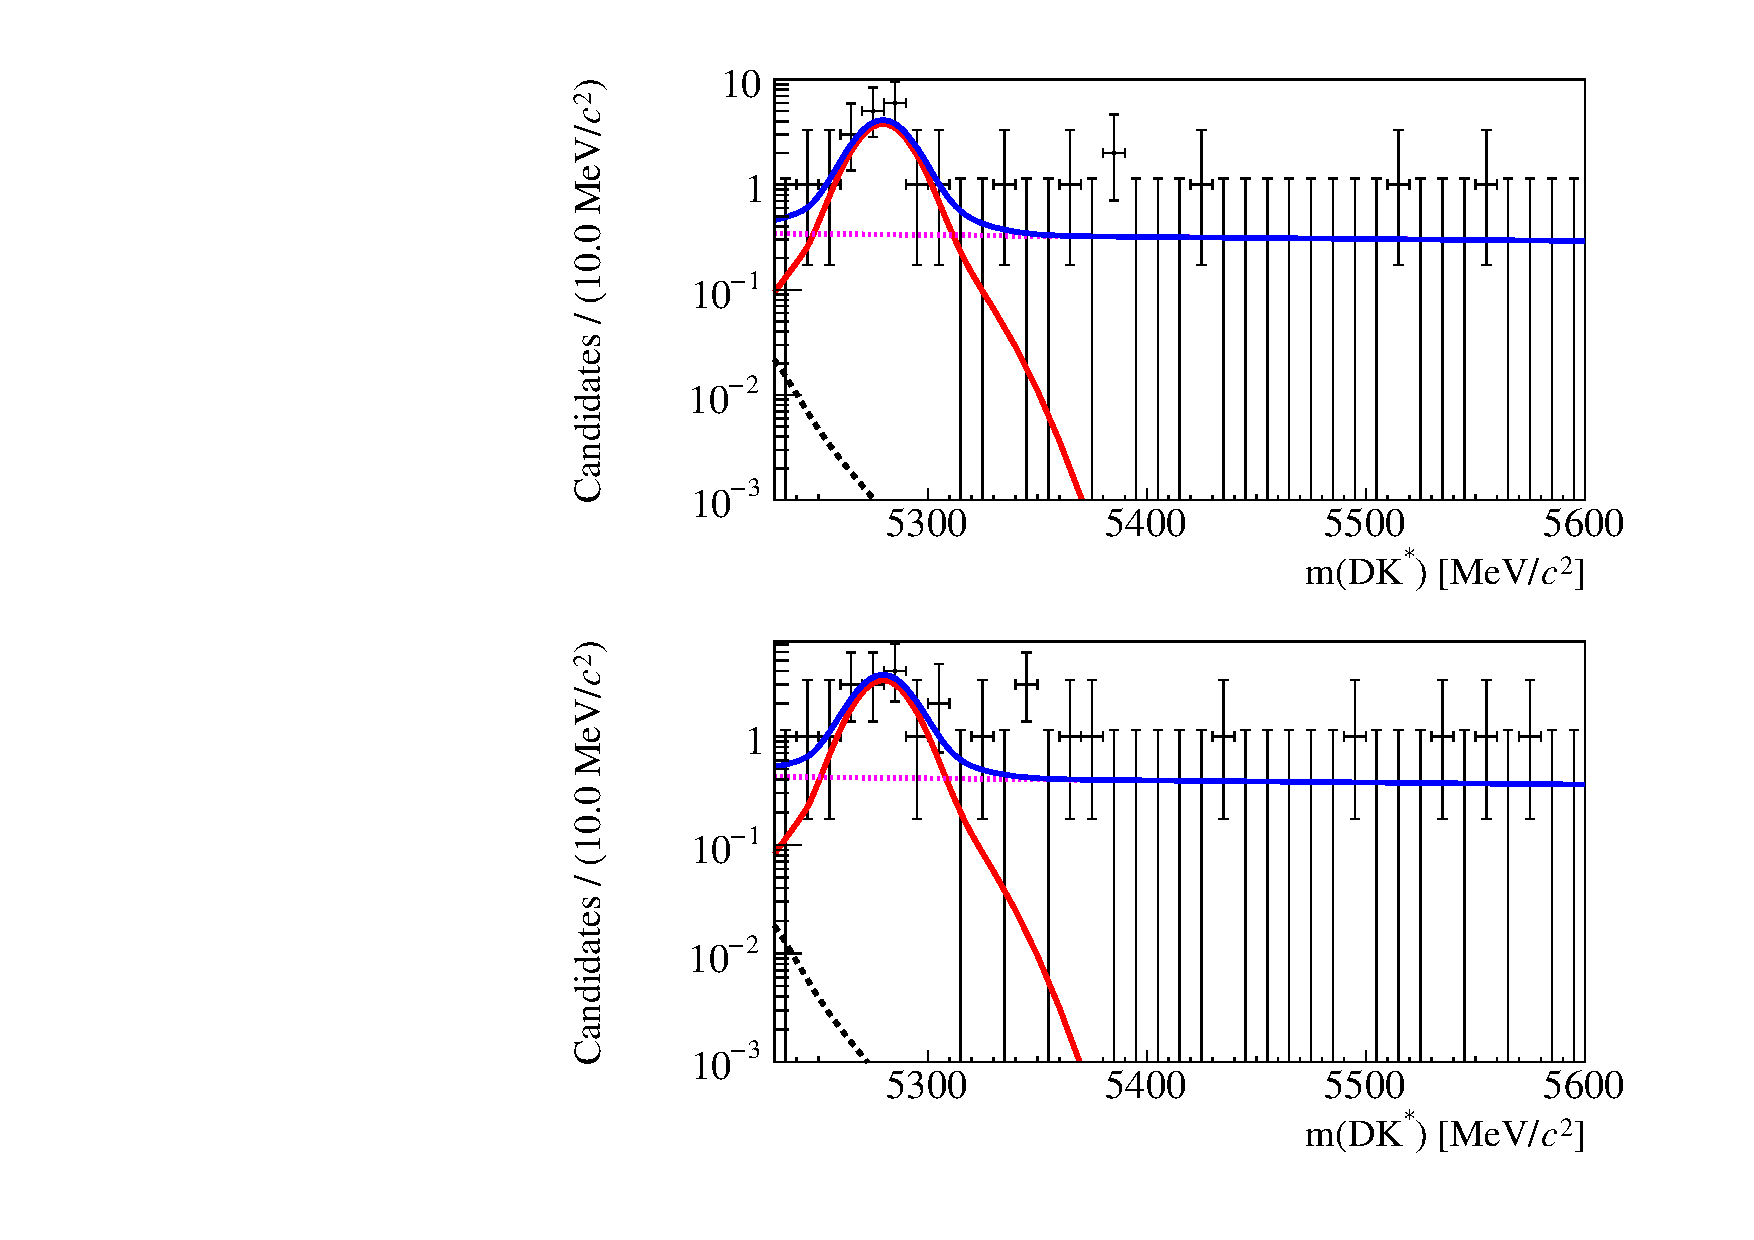
\includegraphics[width=0.3\linewidth]{figures/results/canvaslog_d2pipipipi_LL_run2_log.pdf}}
\hfill
\subfloat[$\pi K\pi\pi$, LL]{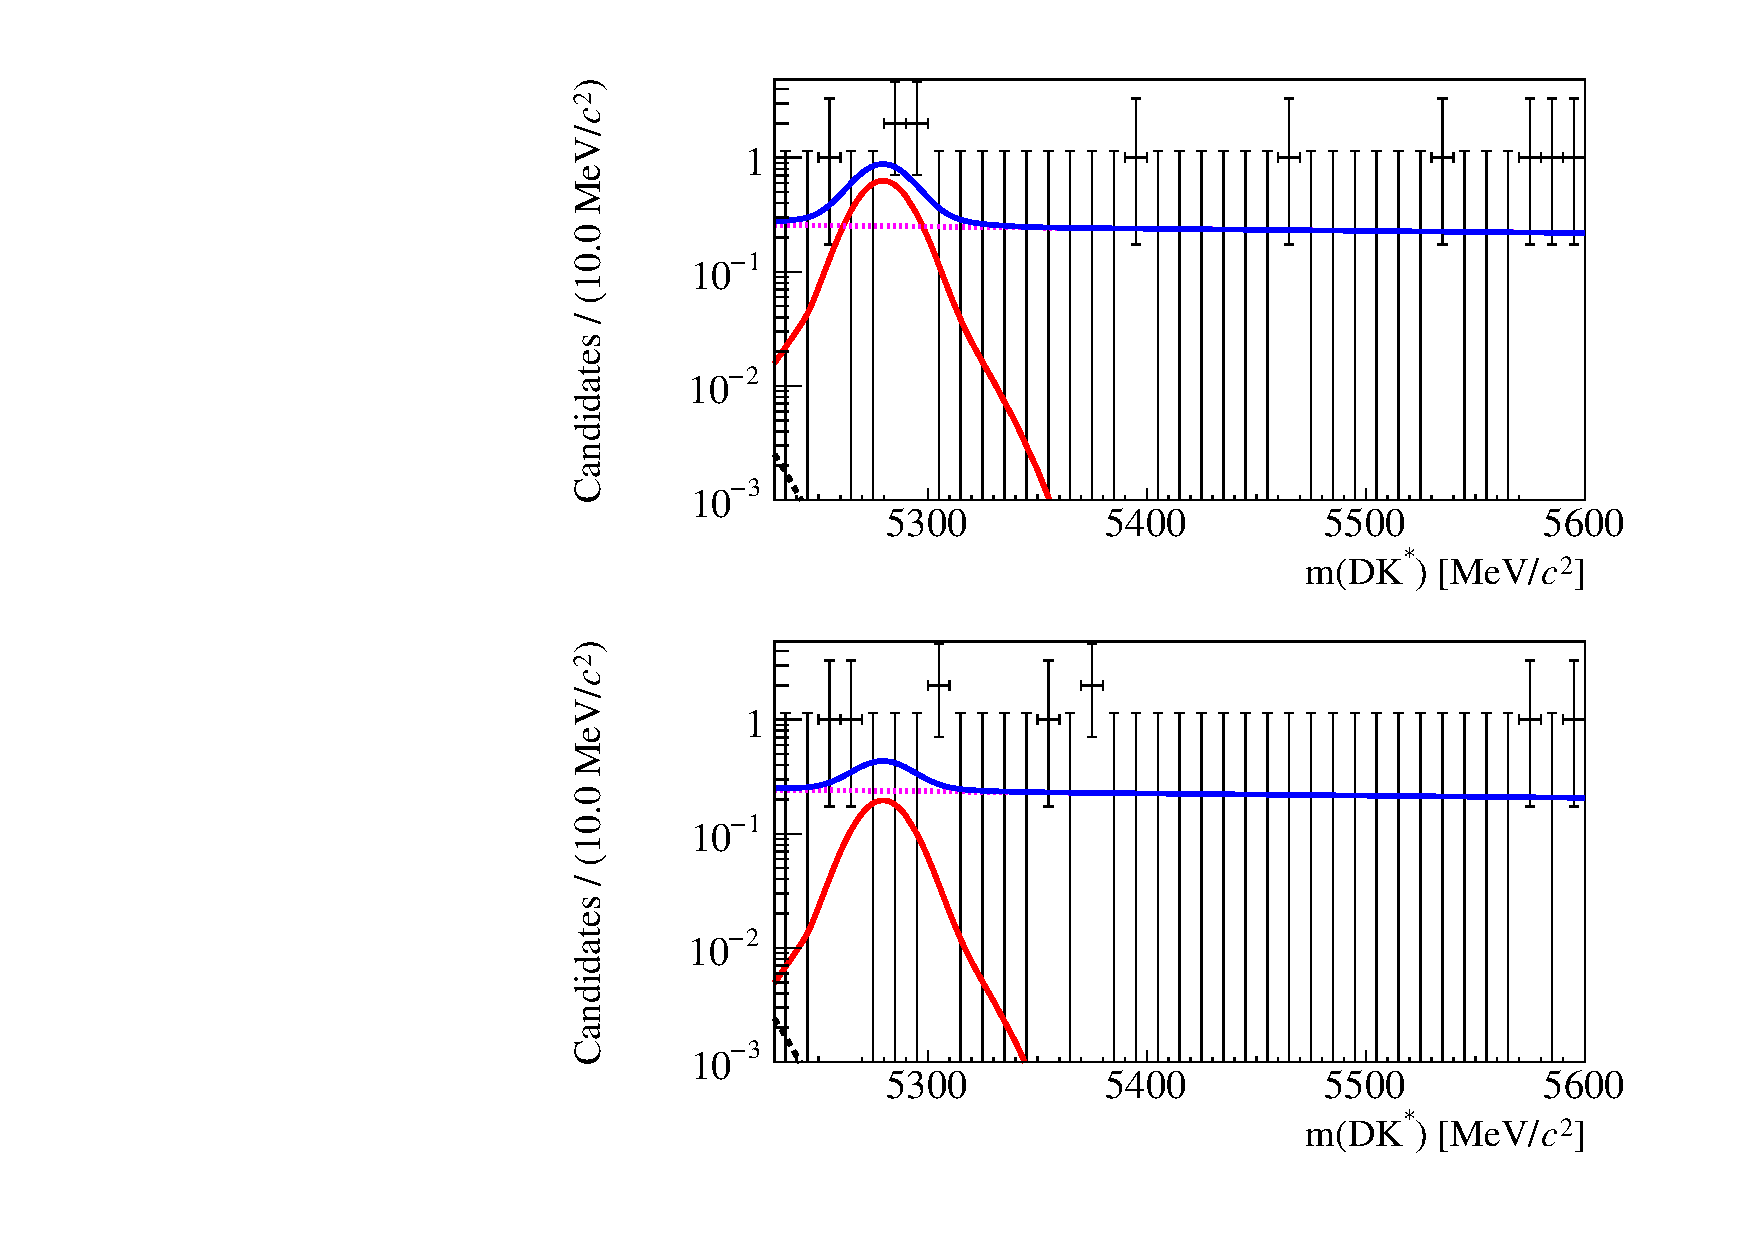
\includegraphics[width=0.3\linewidth]{figures/results/canvaslog_d2pikpipi_LL_run2_log.pdf}}
\hfill
\subfloat[$K\pi\pi\pi$, DD]{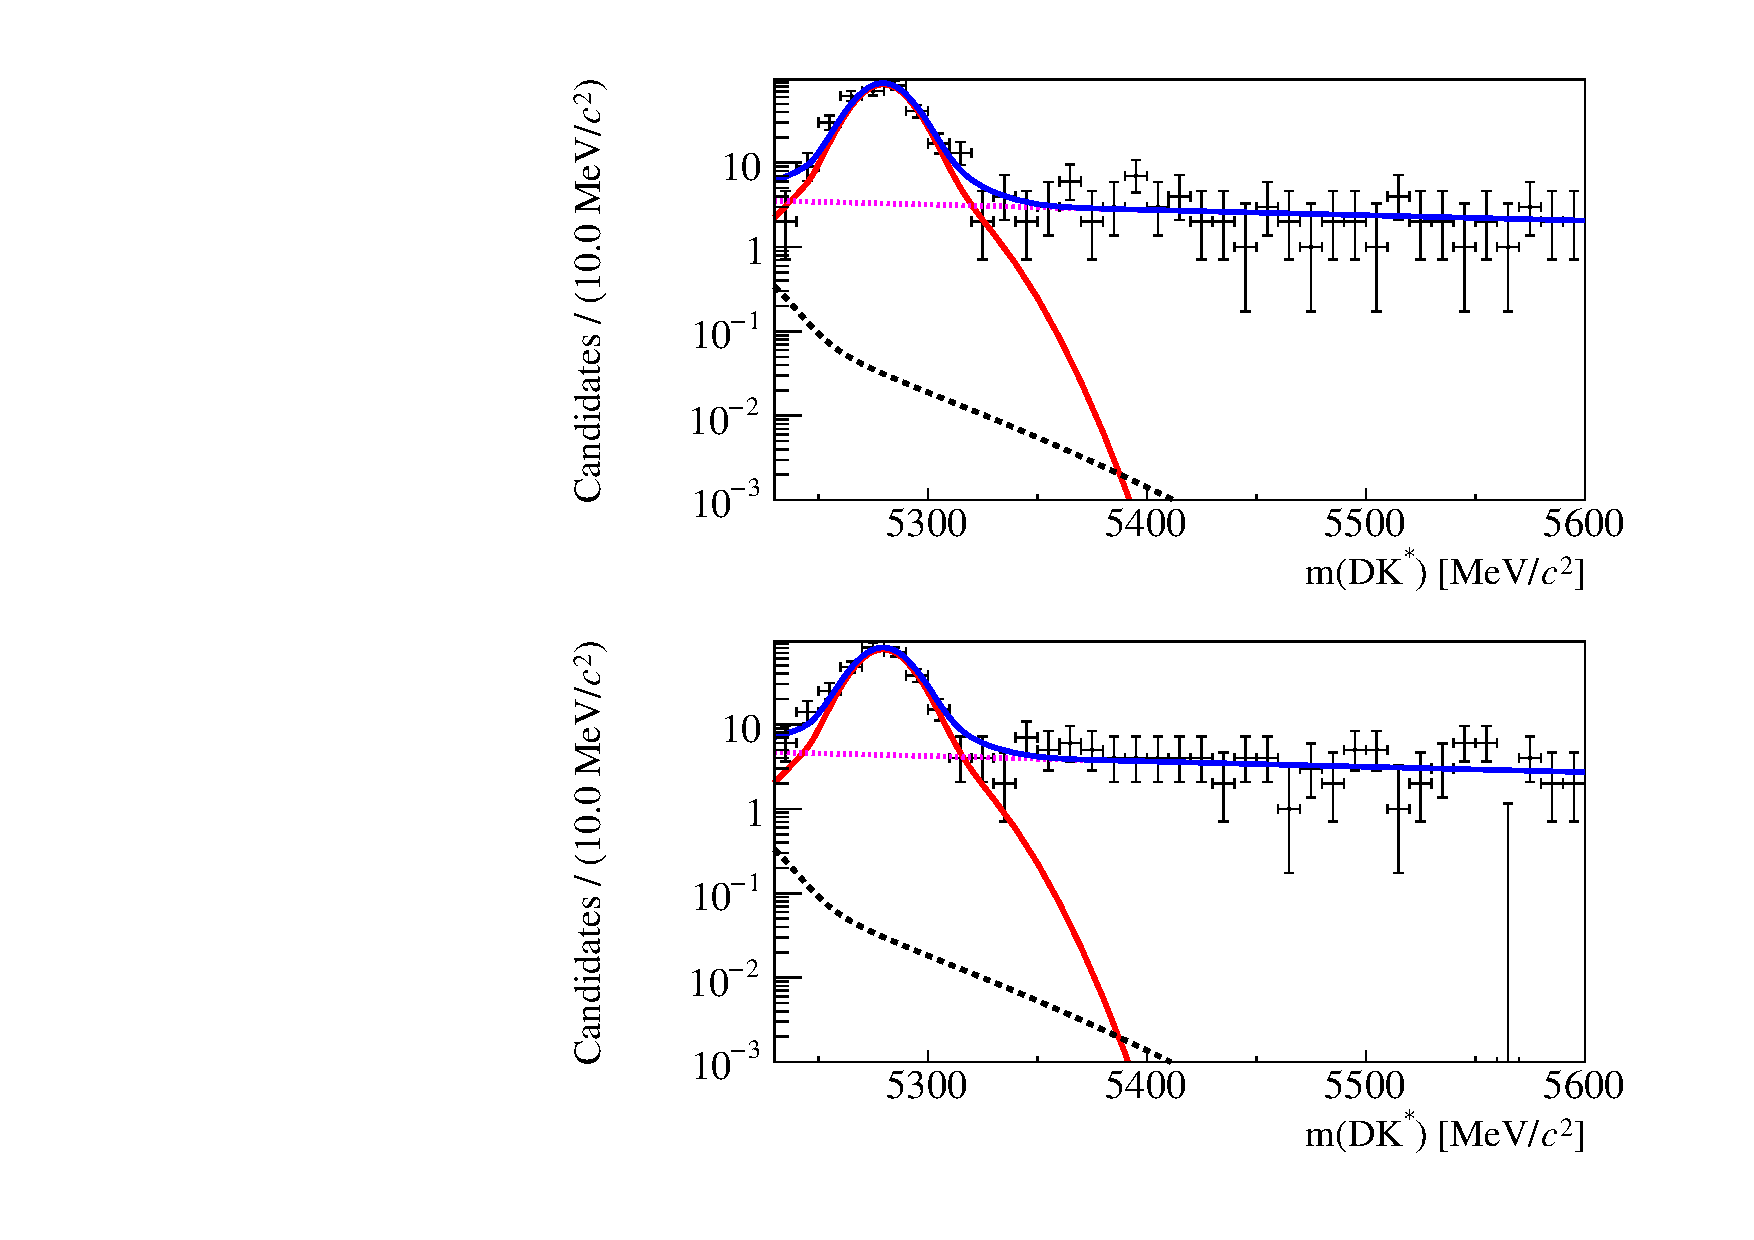
\includegraphics[width=0.3\linewidth]{figures/results/canvaslog_d2kpipipi_DD_run2_log.pdf}}
\hfill
\subfloat[$\pi\pi\pi\pi$, DD]{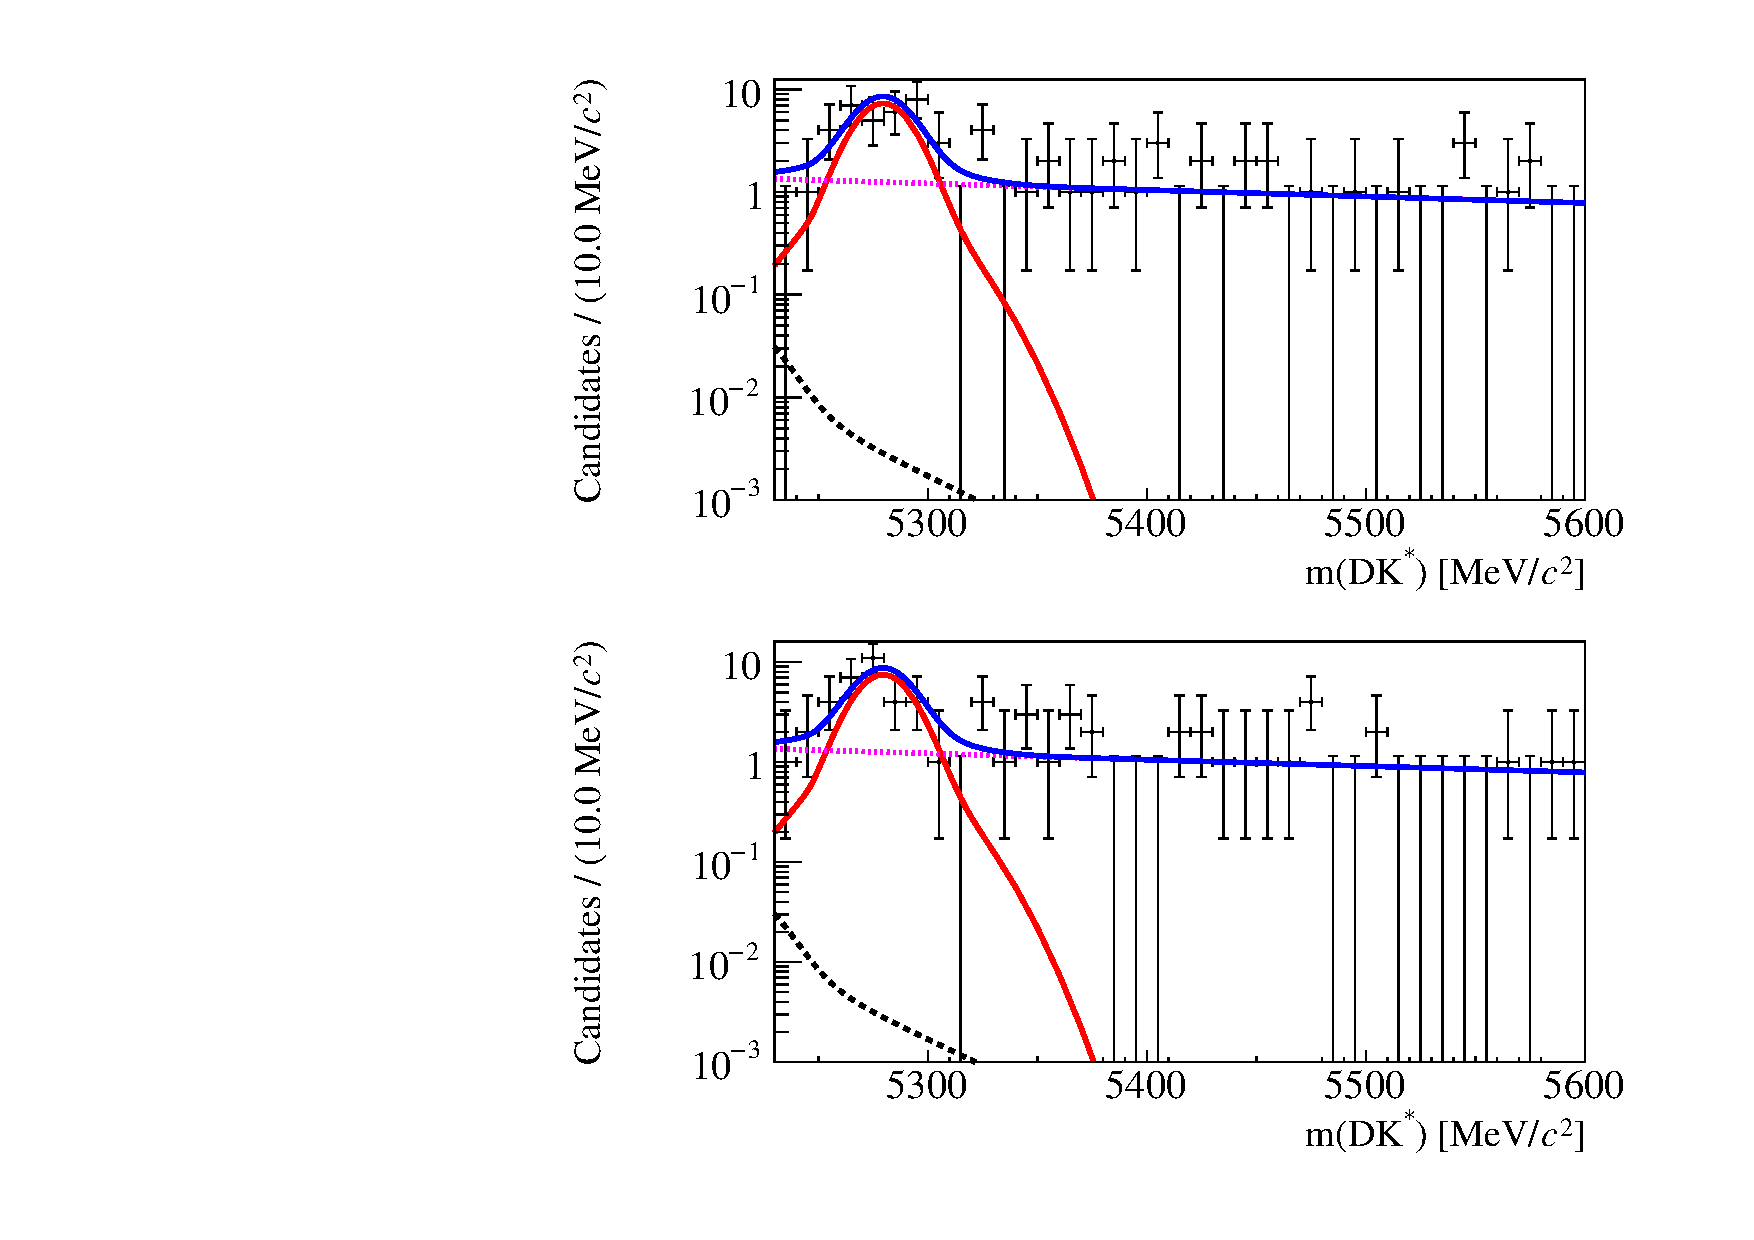
\includegraphics[width=0.3\linewidth]{figures/results/canvaslog_d2pipipipi_DD_run2_log.pdf}}
\hfill
\subfloat[$\pi K\pi\pi$, DD]{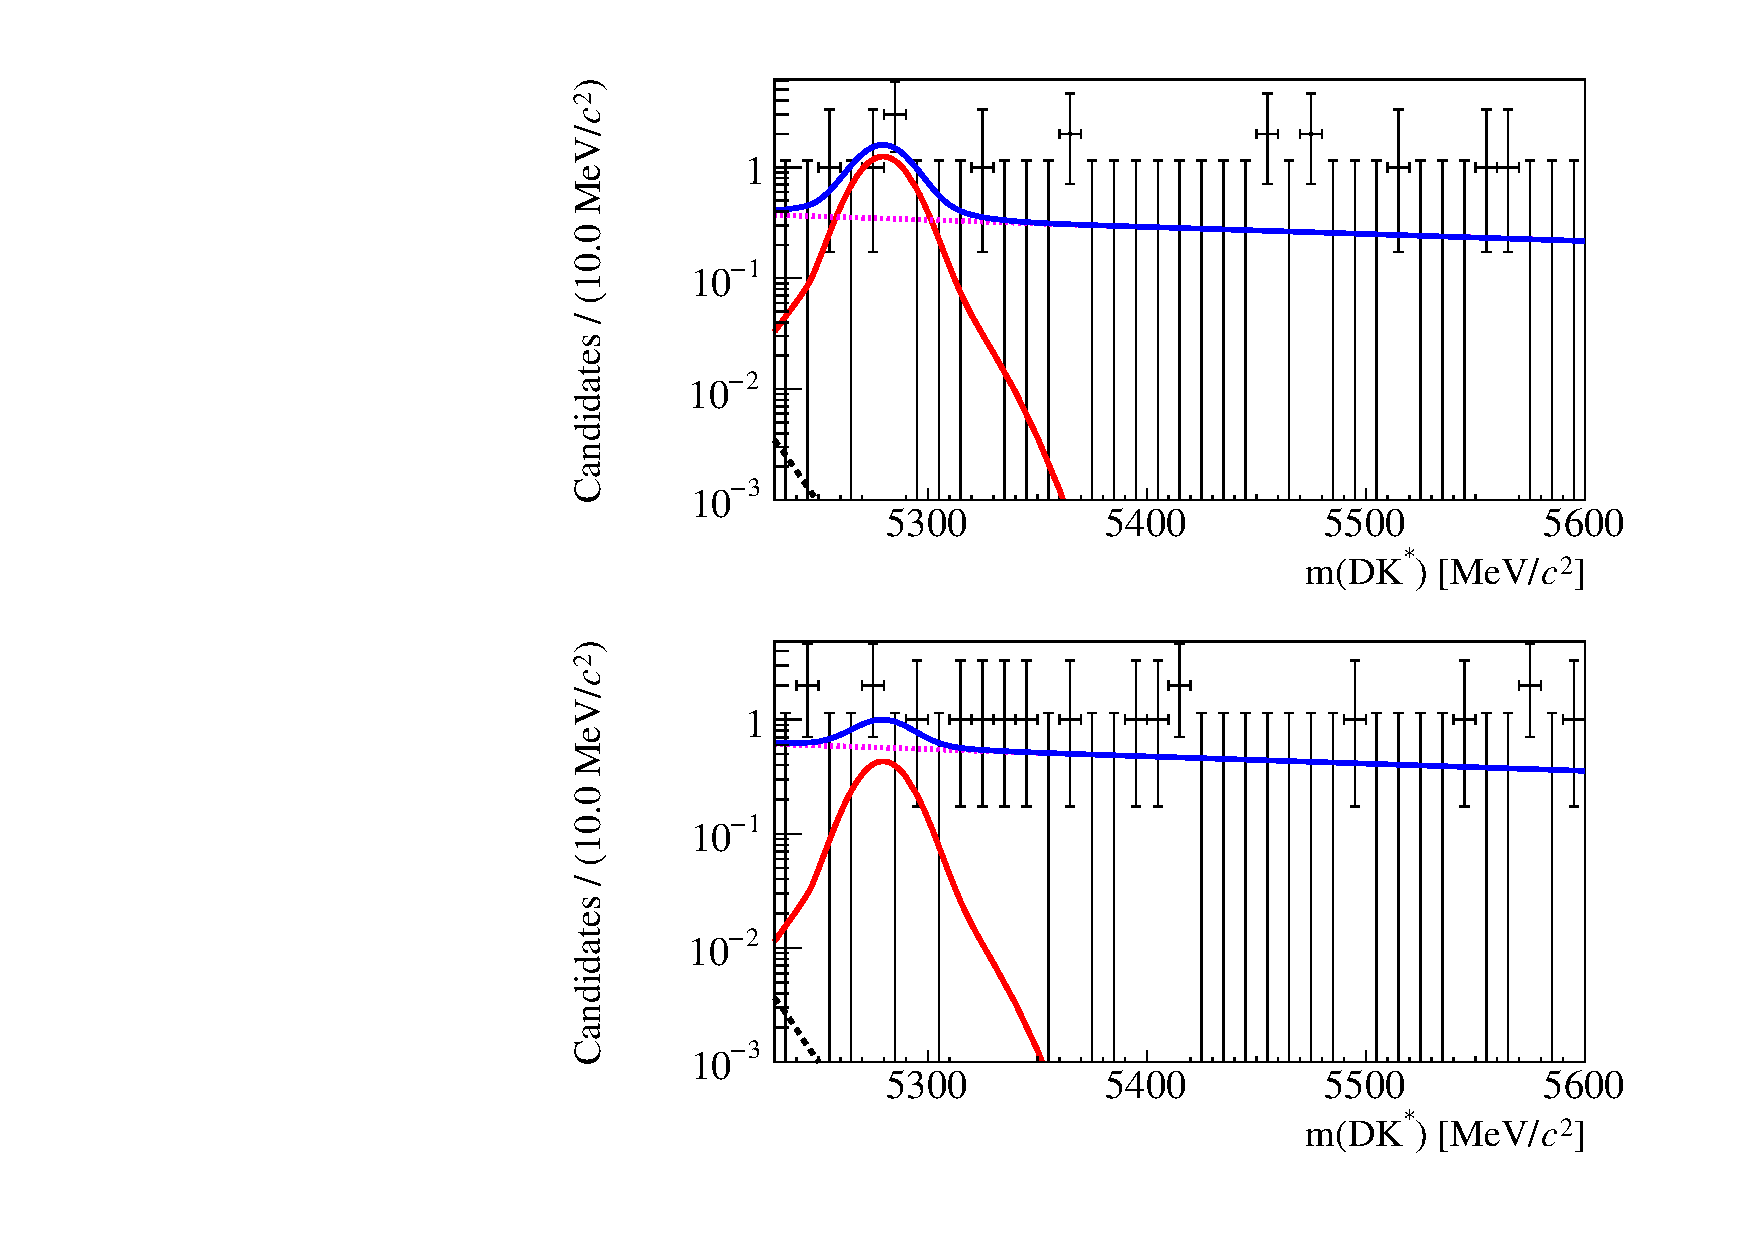
\includegraphics[width=0.3\linewidth]{figures/results/canvaslog_d2pikpipi_DD_run2_log.pdf}}
\caption{Results of the simultaneous fit for Run 1 data for 4-body modes. In each pair the top plot is for \Bp decays and the bottom plot is for \Bm decays.}
\label{datafit4bodyRun2}
\end{sidewaysfigure}

\clearpage
